\documentclass[11pt,a4paper]{article}

% ============================================================
% PACKAGES
% ============================================================
\usepackage[T1]{fontenc}
\usepackage[utf8]{inputenc}
\usepackage{textcomp}
\usepackage[expansion=false]{microtype}
\usepackage{parskip}
\usepackage[a4paper,margin=2.3cm,headheight=14pt]{geometry}
\usepackage{xcolor}
\usepackage{amsmath}
\usepackage{amssymb}
\usepackage{booktabs}
\usepackage{longtable}
\usepackage{array}
\usepackage{enumitem}
\usepackage{fancyhdr}
\usepackage{titlesec}
\usepackage[most]{tcolorbox}
\usepackage{listings}
\usepackage{caption}
\usepackage{hyperref}
\usepackage{tikz}
\usetikzlibrary{arrows.meta, positioning, matrix, calc, shapes.geometric, fit}

% Ragged-right paragraph columns avoid stretched spacing in narrow tables.
\newcolumntype{L}[1]{>{\raggedright\arraybackslash}p{#1}}

% ============================================================
% COLOR PALETTE
% ============================================================
\definecolor{excelgreen}{HTML}{217346}
\definecolor{excelgreenlight}{HTML}{E9F3EE}
\definecolor{pythonblue}{HTML}{1F5C8B}
\definecolor{pythonbluelight}{HTML}{E8F1F8}
\definecolor{pythonyellow}{HTML}{B8860B}
\definecolor{sqlorange}{HTML}{B0521A}
\definecolor{sqlorangelight}{HTML}{FBEEE4}
\definecolor{keyblue}{HTML}{1B4F72}
\definecolor{keybluelight}{HTML}{EAF2F8}
\definecolor{tipgreen}{HTML}{1E7A46}
\definecolor{tipgreenlight}{HTML}{EAF7EF}
\definecolor{warnred}{HTML}{922B21}
\definecolor{warnredlight}{HTML}{FDEDEC}
\definecolor{codegray}{HTML}{F5F5F5}
\definecolor{rulegray}{HTML}{888888}
\definecolor{vbapurple}{HTML}{5C2D91}
\definecolor{vbapurplelight}{HTML}{F2EEF8}

% ============================================================
% HEADER / FOOTER
% ============================================================
\pagestyle{fancy}
\fancyhf{}
\renewcommand{\headrulewidth}{0.4pt}
\fancyhead[L]{\small\textcolor{rulegray}{Excel for Finance --- The Professional Handbook}}
\fancyhead[R]{\small\textcolor{rulegray}{Module 2: Making Excel Professional}}
\fancyfoot[C]{\small\thepage}

% ============================================================
% SECTION STYLING
% ============================================================
\titleformat{\section}
  {\normalfont\Large\bfseries\color{excelgreen}}
  {\thesection}{0.6em}{}[{\color{excelgreen}\titlerule}]
\titleformat{\subsection}
  {\normalfont\large\bfseries\color{keyblue}}
  {\thesubsection}{0.6em}{}
\titleformat{\subsubsection}
  {\normalfont\bfseries\color{black}}
  {\thesubsubsection}{0.6em}{}

% ============================================================
% CODE LISTING STYLES
% ============================================================
\lstdefinestyle{pythonstyle}{
  language=Python,
  backgroundcolor=\color{pythonbluelight},
  basicstyle=\ttfamily\small,
  keywordstyle=\color{pythonblue}\bfseries,
  stringstyle=\color{tipgreen},
  commentstyle=\color{rulegray}\itshape,
  numbers=left,
  numberstyle=\tiny\color{rulegray},
  numbersep=8pt,
  frame=single,
  rulecolor=\color{pythonblue!40},
  framerule=0.4pt,
  breaklines=true,
  showstringspaces=false,
  tabsize=4,
  xleftmargin=2pt,
  framexleftmargin=6pt,
  aboveskip=8pt,
  belowskip=8pt
}

\lstdefinestyle{sqlstyle}{
  language=SQL,
  backgroundcolor=\color{sqlorangelight},
  basicstyle=\ttfamily\small,
  keywordstyle=\color{sqlorange}\bfseries,
  stringstyle=\color{tipgreen},
  commentstyle=\color{rulegray}\itshape,
  numbers=left,
  numberstyle=\tiny\color{rulegray},
  numbersep=8pt,
  frame=single,
  rulecolor=\color{sqlorange!40},
  framerule=0.4pt,
  breaklines=true,
  showstringspaces=false,
  tabsize=4,
  xleftmargin=2pt,
  framexleftmargin=6pt,
  aboveskip=8pt,
  belowskip=8pt
}

\lstdefinestyle{excelstyle}{
  backgroundcolor=\color{excelgreenlight},
  basicstyle=\ttfamily\small\color{black},
  frame=single,
  rulecolor=\color{excelgreen!50},
  framerule=0.4pt,
  breaklines=true,
  showstringspaces=false,
  xleftmargin=2pt,
  framexleftmargin=6pt,
  aboveskip=8pt,
  belowskip=8pt
}

\lstdefinestyle{vbastyle}{
  backgroundcolor=\color{vbapurplelight},
  basicstyle=\ttfamily\small\color{black},
  numbers=left,
  numberstyle=\tiny\color{rulegray},
  numbersep=8pt,
  frame=single,
  rulecolor=\color{vbapurple!50},
  framerule=0.4pt,
  breaklines=true,
  showstringspaces=false,
  tabsize=4,
  xleftmargin=2pt,
  framexleftmargin=6pt,
  aboveskip=8pt,
  belowskip=8pt
}

% ============================================================
% CALLOUT BOXES
% ============================================================
\newtcolorbox{keyconcept}[1][Key Concept]{
  colback=keybluelight, colframe=keyblue, coltitle=white,
  fonttitle=\bfseries, title=#1, boxrule=0.8pt, arc=2pt,
  left=6pt, right=6pt, top=4pt, bottom=4pt
}

\newtcolorbox{financeapp}[1][Finance Application]{
  colback=excelgreenlight, colframe=excelgreen, coltitle=white,
  fonttitle=\bfseries, title=#1, boxrule=0.8pt, arc=2pt,
  left=6pt, right=6pt, top=4pt, bottom=4pt
}

\newtcolorbox{protip}[1][Pro Tip]{
  colback=tipgreenlight, colframe=tipgreen, coltitle=white,
  fonttitle=\bfseries, title=#1, boxrule=0.8pt, arc=2pt,
  left=6pt, right=6pt, top=4pt, bottom=4pt
}

\newtcolorbox{pitfall}[1][Common Pitfall]{
  colback=warnredlight, colframe=warnred, coltitle=white,
  fonttitle=\bfseries, title=#1, boxrule=0.8pt, arc=2pt,
  left=6pt, right=6pt, top=4pt, bottom=4pt
}

\newtcolorbox{formulasyntax}[1][Formula Syntax]{
  colback=white, colframe=excelgreen, coltitle=white,
  fonttitle=\bfseries, title=#1, boxrule=1pt, arc=2pt,
  left=6pt, right=6pt, top=4pt, bottom=4pt
}

% shortcut key style
\newcommand{\key}[1]{\texttt{\colorbox{black!8}{\textbf{#1}}}}

% ============================================================
% HYPERREF SETUP
% ============================================================
\hypersetup{
  colorlinks=true,
  linkcolor=keyblue,
  citecolor=keyblue,
  urlcolor=pythonblue,
  pdftitle={Excel for Finance -- Module 2: Making Excel Professional},
  pdfauthor={Finance \& Analytics Study Notes},
}

\setlist[itemize]{leftmargin=1.4em}
\setlist[enumerate]{leftmargin=1.6em}

% ============================================================
% DOCUMENT
% ============================================================
\begin{document}
\pagenumbering{roman}
\hypersetup{pageanchor=false}

% -------------------- TITLE PAGE --------------------
\begin{titlepage}
\centering
\vspace*{1.5cm}
{\Huge\bfseries\color{excelgreen} Excel for Finance}\\[0.4cm]
{\Large The Complete Professional Handbook}\\[1.2cm]
{\huge\bfseries Module 2}\\[0.3cm]
{\LARGE Making Excel Professional}\\[0.15cm]
{\large Optimisation, Macros \& VBA, Absolute/Relative References,\\ Named Ranges, Data Validation --- with Python and SQL Equivalents}\\[2cm]

\begin{tcolorbox}[colback=excelgreenlight, colframe=excelgreen, width=0.8\textwidth, arc=3pt, before upper=\raggedright]
\textbf{Companion modules in this handbook:}
\begin{itemize}[leftmargin=1.5em]
  \item \textbf{Module 1} --- Excel Foundations: Interface, Data \& Number Formatting, Formula Fundamentals, Shortcuts
  \item \textbf{Module 2} --- Making Excel Professional: Optimisation, Macros, Absolute/Relative References, Named Ranges, Data Validation \& Custom Formatting \textit{(this document)}
  \item \textbf{Module 3} --- Excel Like a Pro: Conditional Formatting, Logical Functions, Lookup Functions (VLOOKUP/HLOOKUP/XLOOKUP/INDEX-MATCH), Conditional Aggregation, Error Handling, String Functions
\end{itemize}
\end{tcolorbox}

\vfill
{\small Compiled study notes covering the Excel curriculum end-to-end, extended with equivalent Python (\texttt{pandas}, \texttt{openpyxl}) and SQL implementations of every concept, for a tech-background learner building cross-tool fluency in financial analytics.}\\[0.3cm]
{\small \today}
\end{titlepage}

\hypersetup{pageanchor=true}
\tableofcontents
\clearpage
\pagenumbering{arabic}

% ==================================================================
\section{How to Use This Module}
% ==================================================================

This module assumes you have completed Module 1 and can comfortably navigate the Excel interface, format numbers, and write basic formulas with relative references. Everything here builds directly on that foundation. As in Module 1, every topic is explained three times, in three dialects:

\begin{itemize}
  \item \textbf{Excel} --- the native implementation: menu paths, dialog boxes, and keyboard shortcuts, exactly as you would click through them.
  \item \textbf{Python} --- the equivalent using \texttt{openpyxl} (for building/formatting actual \texttt{.xlsx} files programmatically) and \texttt{pandas} (for the data-manipulation mindset that replaces several Excel features entirely).
  \item \textbf{SQL} --- the closest conceptual equivalent, since a surprising number of ``make Excel professional'' features exist to compensate for the fact that a worksheet has none of a database's built-in structure, constraints, or automation.
\end{itemize}

The same recurring boxes from Module 1 appear throughout:

\begin{keyconcept}
A foundational idea you must internalise before moving on --- the ``why'', not just the ``how''.
\end{keyconcept}

\begin{financeapp}
How the concept is specifically used in financial modeling, accounting, or investment analysis.
\end{financeapp}

\begin{protip}
A workflow habit that separates a fast, professional analyst from a slow, error-prone one.
\end{protip}

\begin{pitfall}
A mistake that looks harmless but silently corrupts a financial model.
\end{pitfall}

\begin{formulasyntax}
The precise syntax of a function, code, or dialog setting, written the way Excel itself would present it.
\end{formulasyntax}

% ==================================================================
\section{From ``Works'' to ``Professional'': What This Module Adds}
% ==================================================================

Module 1 got a workbook to \emph{produce correct numbers}. That is necessary but not sufficient. A workbook used in a real finance role also has to survive contact with other humans: a colleague who inherits it six months from now, an auditor who has to trust it, a repetitive monthly task that must not eat an hour every time, and a user who will absolutely, eventually, type the wrong thing into an input cell. This module is about the five specific skills that take a spreadsheet from ``technically correct'' to ``professional'':

\begin{enumerate}
  \item \textbf{Optimisation} --- a workbook that is fast, clean, and configured sensibly, rather than sluggish and visually chaotic.
  \item \textbf{Macros} --- automating a repetitive manual task instead of repeating it fifty times by hand.
  \item \textbf{Absolute vs. Relative References} --- the full \texttt{\$} notation, so formulas copy correctly instead of subtly breaking.
  \item \textbf{Named Ranges} --- replacing fragile, meaningless cell addresses (\texttt{\$B\$4}) with self-documenting names (\texttt{TaxRate}), directly solving the positional-reference fragility flagged in Module 1.
  \item \textbf{Data Validation} --- constraining what a user is allowed to type into a cell, Excel's closest equivalent to a database \texttt{CHECK} constraint.
\end{enumerate}

\begin{keyconcept}[The Common Thread]
Every topic in this module exists to solve the same underlying problem: \textbf{a spreadsheet has no enforced structure}. A database table rejects a row that violates a constraint; a Python function signature rejects the wrong type of argument; a compiled program will not even build if a reference is invalid. A blank Excel cell, by contrast, will accept literally anything, and a formula will happily reference the wrong cell forever without complaint. Named Ranges, Data Validation, and disciplined use of absolute references are three different techniques for manually re-imposing the structure that other tools give you for free. Macros and workbook optimisation are about the other half of ``professional'': performance and repeatability at scale, without the safety net of code being run from source control by a CI pipeline.
\end{keyconcept}

% ==================================================================
\section{Optimising and Professionalising a Workbook}
\label{sec:optimisation}
% ==================================================================

\subsection{Two Different Meanings of ``Optimisation''}

The course label ``Optimisation'' actually bundles two distinct goals that are worth separating in your head, because they use different tools:

\begin{keyconcept}[Cosmetic Optimisation vs. Performance Optimisation]
\textbf{Cosmetic optimisation} makes a workbook \emph{look} clean, readable, and deliberate --- consistent fonts, no stray gridlines, sensibly sized columns, no visual clutter. This is about \emph{trust}: a messy-looking model makes a reader doubt the numbers even when they're correct. \textbf{Performance optimisation} makes a workbook \emph{run} fast even as it grows to thousands of formulas --- calculation mode, avoiding volatile functions, avoiding whole-column references. This is about \emph{usability}: a workbook that takes eleven seconds to recalculate after every keystroke will not get used carefully, however elegant its formulas are. A genuinely professional workbook needs both; this section covers each in turn, plus the Excel Options settings that control both.
\end{keyconcept}

\subsection{Wrap Text vs. the Manual Line Break}

Module 1 introduced \textbf{Wrap Text} (Home tab) as a way to keep long text inside one cell by increasing row height instead of overflowing into the next cell. There is a second, related tool worth knowing precisely:

\begin{formulasyntax}[Manual Line Break]
\key{Alt + Enter} while editing a cell inserts a line break \emph{at the cursor position}, forcing a new line exactly where you choose --- independent of column width. It also automatically turns on Wrap Text for that cell, since the line break would otherwise be invisible.
\end{formulasyntax}

\begin{center}
\begin{tabular}{@{}L{3.6cm}L{4.0cm}L{4.4cm}@{}}
\toprule
\textbf{Tool} & \textbf{Breaks the line} & \textbf{Use when} \\
\midrule
Wrap Text (automatic) & Wherever the column width forces it, re-flowing if the column is resized & The text is one continuous sentence/paragraph and you want it to always fit the current column width \\
\key{Alt+Enter} (manual) & Exactly where you place the cursor, permanently & You are building a multi-line label with deliberate structure, e.g. \texttt{Revenue}\allowbreak\texttt{ (USD, 000s)} on two fixed lines regardless of column width \\
\bottomrule
\end{tabular}
\end{center}

\begin{financeapp}
Two-line column headers --- a metric name on the first line and its unit on the second (\texttt{"EBITDA Margin"} / \texttt{"(\%)"}) --- are a near-universal convention in financial models and are built with \key{Alt+Enter}, not by hoping Wrap Text breaks the line in the right place.
\end{financeapp}

\subsection{Text to Columns: Splitting One Cell of Text into Many}
\label{sec:texttocolumns}

\textbf{Text to Columns} (\textbf{Data} tab $\rightarrow$ \textbf{Text to Columns}) takes a column where each cell contains multiple pieces of information glued together as one text string, and splits it into separate columns --- the single most common ``data came in messy'' fix in Excel.

\begin{formulasyntax}[Text to Columns Wizard --- Three Steps]
\begin{enumerate}
  \item \textbf{Original data type}: \textbf{Delimited} (split wherever a character like a comma, tab, space, or semicolon occurs) or \textbf{Fixed width} (split at fixed character positions you click to define --- for data with no separator character, like a legacy fixed-format bank export where columns 1--10 are always the account number).
  \item \textbf{Delimiters} (Delimited only): choose which character(s) mark a split --- Tab, Semicolon, Comma, Space, or a custom character --- and optionally treat consecutive delimiters as one (important for text with irregular spacing).
  \item \textbf{Column data format}: for each resulting column, choose \textbf{General}, \textbf{Text}, or \textbf{Date} (with the date order, e.g. DMY vs. MDY) --- and a \textbf{Destination} cell for where the split output should start (default overwrites the original column).
\end{enumerate}
\end{formulasyntax}

\begin{center}
\begin{tabular}{@{}L{4.2cm}L{2.6cm}L{4.6cm}@{}}
\toprule
\textbf{Before (one cell)} & \textbf{Delimiter} & \textbf{After (three cells)} \\
\midrule
\texttt{Sharma, Anjali, Mumbai} & Comma & \texttt{Sharma} \textbar\ \texttt{Anjali} \textbar\ \texttt{Mumbai} \\
\texttt{INV-2026-00451} & Custom: \texttt{-} & \texttt{INV} \textbar\ \texttt{2026} \textbar\ \texttt{00451} \\
\texttt{2026-08-15} (as text) & --- (Fixed width or Date column type) & Recognised and re-parsed as an actual date value \\
\bottomrule
\end{tabular}
\end{center}

\begin{protip}[The ``Silent Fix'' for Numbers Stored as Text]
Module 1 flagged \textbf{numbers stored as text} as a silent data-quality trap: such cells look like numbers but are excluded from \texttt{SUM}/\texttt{AVERAGE} without any error. Running \textbf{Text to Columns} on the affected column with \textbf{Delimited} selected but \emph{no} delimiter checked, then clicking \textbf{Finish}, forces Excel to re-parse every cell's content and convert genuine numeric text back into real numbers --- a one-click fix that requires no formula at all.
\end{protip}

\subsection{The Recurring Weakness of Text to Columns}

Text to Columns is a \emph{one-time, one-range} operation: you select a specific range, run the wizard once, and it acts only on the cells you had selected at that moment. It is not a live, self-updating feature the way a formula is --- if five new rows of comma-separated data are pasted in below tomorrow, they will \emph{not} automatically get split; you have to select them and re-run the wizard.

\begin{pitfall}[Why a Recorded ``Text to Columns'' Macro Only Works for a Fixed Number of Rows]
This limitation is the exact reason a \emph{macro} that records a Text to Columns action (\S\ref{sec:macros}) breaks the moment your dataset grows: the macro recorder captures the literal range you had selected while recording --- say \texttt{A1:A4} --- and writes that fixed address into the generated code. Run the same macro next month on a sheet with 40 rows, and it will still only touch \texttt{A1:A4}, silently leaving rows 5--40 unsplit, with no error or warning. Section~\ref{sec:macros} shows exactly how to fix this by editing the recorded code to use a dynamic range instead of a hard-coded one.
\end{pitfall}

\subsection{Removing Visual Clutter: Gridlines and Headings}

Module 1's View tab section introduced toggling \textbf{Headings} and \textbf{Gridlines} on or off. It is worth being precise about \emph{why} a professional deliverable almost always has them off:

\begin{itemize}
  \item \textbf{Gridlines} (\textbf{View} tab $\rightarrow$ uncheck \textbf{Gridlines}) are a screen aid for building a sheet, not part of the finished product. A dashboard, summary report, or printed statement with gridlines visible looks like an unfinished worksheet rather than a designed document --- professional models instead use deliberate \textbf{borders} (Home tab $\rightarrow$ Borders) only where a visual boundary is actually meaningful (under a subtotal, around an input box).
  \item \textbf{Row/Column Headings} (the grey \texttt{A B C\ldots} / \texttt{1 2 3\ldots} bars) are similarly a building aid. Turning them off (same \textbf{View} tab checkbox) is standard for a polished dashboard tab, though they are normally left \emph{on} for a working calculation tab where you still need to reference cell addresses while auditing.
  \item These two settings are \textbf{per-worksheet}, not per-workbook --- a common workbook pattern is gridlines/headings \emph{off} on a front-facing ``Dashboard'' or ``Summary'' tab, and \emph{on} for the underlying ``Calculations'' or ``Data'' tabs the analyst still works in directly.
\end{itemize}

\begin{pitfall}[Screen Gridlines vs. Printed Gridlines Are Two Separate Settings]
Turning off \textbf{View $\rightarrow$ Gridlines} only affects what you see on screen. Whether gridlines appear on a \emph{printed} page (or a PDF export) is a separate checkbox: \textbf{Page Layout} tab $\rightarrow$ \textbf{Sheet Options} $\rightarrow$ \textbf{Gridlines} $\rightarrow$ \textbf{Print}. It is entirely possible (and a common mistake) to have a clean-looking screen that still prints with gridlines, or vice versa.
\end{pitfall}

\subsection{Row Height and Column Width}

\begin{center}
\begin{tabular}{@{}L{3.8cm}L{4.0cm}L{4.6cm}@{}}
\toprule
\textbf{Method} & \textbf{How} & \textbf{Best for} \\
\midrule
Auto-fit by double-click & Double-click the border between two column letters (or row numbers) & Quickly sizing a column to exactly fit its widest current entry \\
Manual exact size & Right-click a column/row header $\rightarrow$ \textbf{Column Width}/\textbf{Row Height} $\rightarrow$ type a number & Making several columns \emph{identically} sized for a clean grid look (auto-fit alone rarely produces matching widths) \\
Format menu & \textbf{Home} $\rightarrow$ \textbf{Format} $\rightarrow$ \textbf{AutoFit Column Width} / \textbf{AutoFit Row Height} & Applying auto-fit to a multi-column/row selection at once \\
\bottomrule
\end{tabular}
\end{center}

\begin{protip}[Standard Widths for Financial Models]
Many banking and equity-research templates set every input/label column to a uniform width (a common convention is roughly 9--11 characters, i.e. just wide enough for a value like \texttt{(1,234.5)}) rather than auto-fitting each column independently --- the uniformity itself is what reads as ``professional'', even more than the exact number chosen.
\end{protip}

\subsection{Fonts: Consistency Over Decoration}

\begin{keyconcept}
Unlike a Word document or a slide deck, a spreadsheet's font choice is not primarily about aesthetics --- it is about \textbf{numeric legibility and consistency}. A single font, single size, applied uniformly, is what allows a reader's eye to scan a column of numbers instantly for outliers. Calibri and Arial are the two overwhelmingly dominant choices in professional finance because both render numerals with clearly distinct digit shapes and consistent character width at small sizes; a workbook mixing three or four different fonts reads as unplanned, however individually reasonable each font is.
\end{keyconcept}

A typical convention: one base font (e.g. Arial 10 or Calibri 11) for the entire workbook, with \textbf{bold} reserved for headers/totals and \textbf{font colour} reserved for the input-cell convention (blue = hard-coded input, black = formula, green = link to another sheet) rather than for decoration.

\subsection{Excel Options: Configuring the Application Itself}
\label{sec:exceloptions}

Everything so far has configured a \emph{worksheet}. \textbf{File $\rightarrow$ Options} configures \emph{Excel itself}, and several settings here directly affect how professional and efficient your day-to-day workbook building is.

\begin{center}
\begin{tabular}{@{}L{2.6cm}L{3.2cm}L{6.0cm}@{}}
\toprule
\textbf{Tab} & \textbf{Setting} & \textbf{Why it matters} \\
\midrule
General & Default font \& size for new workbooks & Locks in the font-consistency convention above at the source, instead of reformatting every new workbook by hand. \\
Formulas & Workbook Calculation: Automatic / Automatic Except for Data Tables / Manual & Covered in depth in \S\ref{sec:calcmode} --- the single biggest lever for performance on a large model. \\
Formulas & R1C1 reference style & Switches cell addressing from \texttt{A1}-style to \texttt{R1C1} (Row 1, Column 1) notation --- rarely used day-to-day, but this \emph{is} the addressing style VBA's recorded code uses internally (\S\ref{sec:macros}), so recognising it helps when reading macro code. \\
Formulas & Enable iterative calculation & Required to allow deliberate \textbf{circular references} (Module 1, \S\,``Common Pitfalls'') to resolve instead of erroring --- used sparingly, e.g. for a debt schedule where interest expense depends on a cash balance that itself depends on interest expense. \\
Save & AutoRecover interval; default file format & Set the autosave interval low (e.g. 5 minutes) for large models where a crash is costly; default format should be \texttt{.xlsx} (or \texttt{.xlsm} if the workbook always carries macros, \S\ref{sec:macros}). \\
Advanced & After pressing Enter, move selection & Direction the active cell moves after \key{Enter} --- set to \textbf{Down} for entering a column of data quickly, or disabled entirely for formula auditing. \\
Advanced & Show a zero in cells that have a zero value & Unchecking this displays zero-value cells as blank --- common in presentation-ready financial statement tabs where a literal \texttt{0} is visually noisier than empty space. \\
Customize Ribbon & Developer tab checkbox & \textbf{Required} to access macro recording, the VBA editor, and Data Validation's more advanced options --- covered next in \S\ref{sec:macros}. \\
Trust Center & Macro Settings & Controls whether macros run automatically, prompt, or are blocked outright when a workbook is opened --- see the security note in \S\ref{sec:macrosecurity}. \\
\bottomrule
\end{tabular}
\end{center}

\subsection{Opening a Specific Workbook Automatically at Startup}
\label{sec:xlstart}

\begin{formulasyntax}[The XLSTART Folder]
Any workbook, template, or workspace file placed inside Excel's \textbf{XLSTART} folder is opened automatically, every time Excel launches. On Windows, the default per-user location is:
\begin{center}
\texttt{C:\textbackslash Users\textbackslash\textless username\textgreater\textbackslash AppData\textbackslash Roaming\textbackslash Microsoft\textbackslash Excel\textbackslash XLSTART}
\end{center}
An \textbf{alternate startup folder} can additionally be specified at \textbf{File $\rightarrow$ Options $\rightarrow$ Advanced $\rightarrow$ General $\rightarrow$ ``At startup, open all files in:''}, useful when the default AppData path is inconvenient to reach or you want a shared, version-controlled startup folder.
\end{formulasyntax}

This is also precisely how the \textbf{Personal Macro Workbook} (\texttt{PERSONAL.XLSB}) makes your macros available in \emph{every} workbook you open, not just the one they were recorded in --- it is simply a workbook that lives in \texttt{XLSTART} and is therefore always loaded (see \S\ref{sec:personalmacro}).

\begin{pitfall}[Auto-Run Macros on Startup]
If a workbook placed in \texttt{XLSTART} contains a macro named exactly \texttt{Auto\_Open}, that macro executes automatically every time Excel starts --- powerful for setting up a standard environment, but also the reason security software and Excel's own Trust Center are cautious about auto-opened, macro-enabled files from an untrusted source (\S\ref{sec:macrosecurity}).
\end{pitfall}

\subsection{Calculation Mode and Performance Optimisation}
\label{sec:calcmode}

As a model grows past a few thousand formulas, \emph{when} Excel recalculates starts to matter as much as \emph{what} it calculates.

\begin{formulasyntax}[Calculation Modes --- Formulas Tab $\rightarrow$ Calculation Options]
\begin{itemize}
  \item \textbf{Automatic} (default): every formula in every open workbook recalculates after \emph{any} change, anywhere.
  \item \textbf{Automatic Except for Data Tables}: everything recalculates automatically \emph{except} What-If Analysis Data Tables, which are often the single most expensive object in a model (they can force thousands of hidden recalculations) --- a good middle ground.
  \item \textbf{Manual}: nothing recalculates until you explicitly trigger it with \key{F9} (calculate all open workbooks), \key{Shift+F9} (calculate only the active sheet), or \key{Ctrl+Alt+F9} (force a full recalculation of everything, ignoring Excel's usual ``only recalculate what changed'' optimisation --- useful when you suspect a stale cached value).
\end{itemize}
\end{formulasyntax}

\begin{protip}[When to Switch to Manual]
On a large financial model (multi-tab DCFs, three-statement models, anything with thousands of formulas or several Data Tables), switching to \textbf{Manual} calculation while actively editing assumptions --- then pressing \key{F9} deliberately once changes are finished --- can turn a multi-second freeze after every keystroke into an instant, responsive editing experience. The discipline this requires (remembering to recalculate before trusting a displayed number) is the trade-off; Excel shows \textbf{``Calculate''} in the status bar as a reminder that a recalculation is pending.
\end{protip}

\begin{pitfall}[Volatile Functions]
A \textbf{volatile} function forces \emph{itself and everything that depends on it} to recalculate on \emph{every single} recalculation event, even when none of its actual inputs changed. The most common volatile functions are \texttt{NOW()}, \texttt{TODAY()}, \texttt{RAND()}, \texttt{RANDBETWEEN()}, \texttt{OFFSET()}, \texttt{INDIRECT()}, and \texttt{CELL()}/\texttt{INFO()} in some argument forms. A model with a few hundred \texttt{OFFSET}-based dynamic ranges can become dramatically slower than an equivalent model built with \texttt{INDEX} (which is \emph{not} volatile and returns a reference just as flexibly) --- a swap worth knowing about even before Module 3 formally introduces \texttt{INDEX}/\texttt{MATCH}.
\end{pitfall}

\begin{protip}[Other Performance Habits]
Beyond calculation mode: avoid referencing \emph{entire columns} (\texttt{=SUM(A:A)}) when a bounded range (\texttt{=SUM(A2:A10000)}) will do, since a whole-column reference forces Excel to consider all 1,048,576 rows on every recalculation; prefer helper columns with simple formulas over one deeply nested formula repeated across a sheet (simple formulas repeated are cheaper for Excel's calculation engine, and dramatically easier for a human to audit); and keep formatting (especially conditional formatting rules) as narrow as the actual data range rather than applied to whole rows/columns ``just in case''.
\end{protip}

\subsection{Cross-Tool Translation: Python and SQL}

\begin{center}
\begin{tabular}{@{}L{3.0cm}L{4.4cm}L{5.2cm}@{}}
\toprule
\textbf{Excel concept} & \textbf{Python equivalent} & \textbf{Notes} \\
\midrule
Manual calculation mode & Simply not re-running a script until you choose to & Python has no equivalent of an ``always-on reactive engine'' to switch off --- a \texttt{.py} script only computes when you execute it, so this entire lever is unnecessary in Python; it exists in Excel purely because Excel recalculates by default. \\
Avoiding volatile functions & Avoiding an expensive operation inside a loop that re-runs unnecessarily & Same underlying performance principle: do expensive work once, cache the result, and only redo it when a genuine input changed --- vs. recomputing it on every iteration regardless. \\
Text to Columns & \texttt{Series.\allowbreak str.\allowbreak split(delimiter,\allowbreak expand=True)} & Splits a whole pandas column of delimited text into several columns in one vectorised call, applying instantly to every row --- Text to Columns' ``breaks on new rows'' limitation (\S\ref{sec:texttocolumns}) simply does not exist here, since re-running the script naturally covers however many rows the data currently has. \\
Column width / row height & Cosmetic \texttt{openpyxl} properties on the output file & See listing below --- purely presentational, with no equivalent effect on how pandas processes the data itself. \\
\bottomrule
\end{tabular}
\end{center}

\begin{lstlisting}[style=pythonstyle, caption={Text to Columns, the pandas way --- generalises automatically to any number of rows}]
import pandas as pd

df = pd.DataFrame({"full_name": ["Sharma, Anjali", "Verma, Rohit", "Iyer, Kavya"]})

# Splits EVERY row in one call, no matter how many there are --
# unlike the Excel wizard, this never needs to be "re-run" as rows are added.
split_cols = df["full_name"].str.split(", ", expand=True)
df["last_name"], df["first_name"] = split_cols[0], split_cols[1]
print(df)
#          full_name last_name first_name
# 0   Sharma, Anjali     Sharma     Anjali
# 1     Verma, Rohit      Verma      Rohit
# 2     Iyer, Kavya        Iyer      Kavya
\end{lstlisting}

\begin{lstlisting}[style=pythonstyle, caption={Cosmetic worksheet optimisation with openpyxl}]
from openpyxl import Workbook

wb = Workbook()
ws = wb.active

# Equivalent of View -> Gridlines (unchecked)
ws.sheet_view.showGridLines = False

# Equivalent of manually setting column width / row height
ws.column_dimensions["A"].width = 18
ws.row_dimensions[1].height = 20

wb.save("clean_dashboard.xlsx")
\end{lstlisting}

SQL has no real analogue for cosmetic optimisation (a table has no font or gridlines), but its \emph{performance}-optimisation story is directly parallel to Excel's calculation-mode discussion:

\begin{lstlisting}[style=sqlstyle, caption={SQL performance optimisation: an index is the closest relative of Excel's calculation-mode discipline}]
-- Without an index, this scans every row in the table every time it runs --
-- the SQL equivalent of a whole-column SUM(A:A) forcing Excel to walk
-- all 1,048,576 rows on every keystroke.
SELECT * FROM monthly_expenses WHERE category = 'Rent';

-- Building an index lets the database jump straight to matching rows
-- instead of scanning the whole table -- conceptually the same payoff
-- as swapping a volatile OFFSET for a non-volatile INDEX in Excel.
CREATE INDEX idx_category ON monthly_expenses (category);
\end{lstlisting}

% ==================================================================
\section{Macros and VBA: Automating Repetitive Tasks}
\label{sec:macros}
% ==================================================================

\subsection{What a Macro Actually Is}

\begin{keyconcept}
A \textbf{macro} is a saved, named sequence of Excel actions that can be replayed on demand --- either by clicking a button, pressing an assigned shortcut, or calling it from other code. Under the hood, every macro is a small program written in \textbf{VBA} (Visual Basic for Applications), Excel's built-in programming language. You do not have to \emph{write} VBA to create a macro: the \textbf{Macro Recorder} watches every click and keystroke you make and automatically generates the equivalent VBA code, which is how most people first encounter macros. This makes a macro conceptually identical to a short Python script that automates a repetitive task --- the difference is that the ``recorder'' writes the first draft of the code for you by literally watching what you did, rather than you writing it from a blank file.
\end{keyconcept}

\subsection{Enabling the Developer Tab}

Macro recording and the VBA editor live on the \textbf{Developer} tab, which is hidden by default.

\begin{formulasyntax}[Enabling Developer]
\textbf{File $\rightarrow$ Options $\rightarrow$ Customize Ribbon} $\rightarrow$ in the right-hand list of main tabs, check the box next to \textbf{Developer} $\rightarrow$ \textbf{OK}. This is a one-time, per-installation setting (\S\ref{sec:exceloptions}).
\end{formulasyntax}

\subsection{Recording a Macro}
\label{sec:recordmacro}

\begin{formulasyntax}[Developer $\rightarrow$ Record Macro]
\begin{enumerate}
  \item \textbf{Macro name}: no spaces allowed (use underscores), must start with a letter.
  \item \textbf{Shortcut key} (optional): assigns \key{Ctrl+\textless letter\textgreater} (or \key{Ctrl+Shift+\textless letter\textgreater}) to run the macro instantly.
  \item \textbf{Store macro in}: \textbf{This Workbook} (macro travels with this file only), \textbf{New Workbook}, or \textbf{Personal Macro Workbook} (macro becomes available in \emph{every} workbook you open --- see \S\ref{sec:personalmacro}).
  \item Click \textbf{OK} --- recording begins immediately. Perform the exact clicks, formatting, formula entries, or menu actions you want automated.
  \item \textbf{Developer $\rightarrow$ Stop Recording} when finished.
\end{enumerate}
\end{formulasyntax}

\begin{pitfall}[Relative vs. Absolute References While Recording]
Next to \textbf{Record Macro} is a toggle button, \textbf{Use Relative References}, and it fundamentally changes what gets recorded --- this is one of the most consequential and least understood settings for anyone recording macros.
\begin{itemize}
  \item \textbf{Off (default, absolute)}: the macro records the \emph{exact cell addresses} you clicked --- ``select \texttt{A1:D4}, apply bold''. Running the macro again always acts on \texttt{A1:D4}, regardless of where your cursor currently is.
  \item \textbf{On (relative)}: the macro records actions \emph{relative to wherever the active cell was when recording started} --- ``select 4 rows down and 3 columns right from the starting cell''. Running the macro again acts relative to \emph{wherever your cursor currently is} when you run it.
\end{itemize}
Neither setting is ``correct'' in general --- absolute is right for a macro that always formats the same fixed report header; relative is right for a macro meant to be run starting from different cells each time (e.g., ``bold whatever row I've currently selected''). Recording with the wrong one selected is the single most common reason a macro that worked once behaves unexpectedly the second time.
\end{pitfall}

\subsection{Saving Macros: the .xlsm File Format}

\begin{pitfall}[Macros Are Silently Discarded by the Standard .xlsx Format]
A plain \texttt{.xlsx} file \textbf{cannot} contain VBA code at all. If you record a macro and then save with \textbf{Ctrl+S} in a workbook still named \texttt{.xlsx}, Excel will pop up a warning and, if you proceed, will strip every macro out of the saved file --- silently, with no further prompt. You must use \textbf{File $\rightarrow$ Save As} and explicitly choose \textbf{Excel Macro-Enabled Workbook (*.xlsm)} as the file type \emph{before} the macro is saved for good.
\end{pitfall}

\begin{center}
\begin{tabular}{@{}L{2.6cm}L{4.6cm}L{5.2cm}@{}}
\toprule
\textbf{Extension} & \textbf{Can contain macros?} & \textbf{Notes} \\
\midrule
\texttt{.xlsx} & No & Standard format; safest to share externally since it cannot carry executable code. \\
\texttt{.xlsm} & Yes & Identical to \texttt{.xlsx} in every other respect; the ``m'' is the only signal that macros are present. \\
\texttt{.xlsb} & Yes (binary) & A binary (non-XML) format, faster to open/save for very large workbooks, and what the Personal Macro Workbook itself uses (\texttt{PERSONAL.XLSB}). \\
\bottomrule
\end{tabular}
\end{center}

\subsection{Macro Security}
\label{sec:macrosecurity}

Because a macro is executable code, Excel treats macro-enabled files with deliberate caution: opening an \texttt{.xlsm} from an untrusted source (downloaded, emailed) typically opens in \textbf{Protected View} with macros disabled and a yellow \textbf{``Enable Content''} bar, which requires an explicit, informed click before any macro can run. \textbf{File $\rightarrow$ Options $\rightarrow$ Trust Center $\rightarrow$ Trust Center Settings $\rightarrow$ Macro Settings} controls the default behaviour (from ``disable all macros with notification'' to ``enable all macros'', the latter strongly discouraged). This caution exists because macros historically have been (and still are) a common vector for malware distributed as seemingly innocuous spreadsheet attachments --- never enable macros in a file from a source you don't trust, and never disable this protection workbook-wide just to remove the prompt.

\subsection{Reading and Editing Recorded VBA Code}
\label{sec:vbaeditor}

\begin{formulasyntax}[Opening the VBA Editor]
\key{Alt+F11} (or \textbf{Developer $\rightarrow$ Visual Basic}) opens the \textbf{VBA Editor}, a separate application window with its own \textbf{Project Explorer} (a tree of every open workbook and its \textbf{Modules}, where recorded macro code lives) and a code-editing pane.
\end{formulasyntax}

\textbf{Worked example.} Recording a macro that bolds a header row and applies a currency number format to \texttt{B2:B6} (absolute references, recorded exactly as described in \S\ref{sec:recordmacro}) produces VBA code that looks like this:

\begin{lstlisting}[style=vbastyle, caption={Recorded macro: format a header row and a fixed range of amounts}]
Sub FormatExpenseReport()
'
' FormatExpenseReport Macro
'

    Range("A1:B1").Select
    Selection.Font.Bold = True
    Range("B2:B6").Select
    Selection.NumberFormat = "$#,##0.00;[Red](#,##0.00)"
    Range("A1").Select
End Sub
\end{lstlisting}

\begin{keyconcept}[Reading Recorded Code]
Every line follows the same pattern the recorder always uses: \textbf{select something, then act on the Selection}. \texttt{Range("A1:B1").Select} is the VBA equivalent of clicking and dragging across those cells; \texttt{Selection.Font.Bold = True} is the equivalent of clicking the Bold button. This ``select, then act'' style is verbose and not how a human VBA programmer would write it from scratch (you can act on a \texttt{Range} object directly, without selecting it first), but it is exactly how the recorder works, because the recorder can only capture actions performed \emph{on whatever is currently selected} --- it has no concept of your underlying intent, only of the clicks you physically made.
\end{keyconcept}

\subsection{The ``Only Works for 4 Rows'' Problem, Solved}
\label{sec:macrofix}

This is the single most important limitation to understand about recorded macros, and it applies to \emph{any} recorded action, not just Text to Columns.

\begin{pitfall}[Why the Recorder Always Hard-Codes a Fixed Range]
Suppose you record a macro that runs \textbf{Text to Columns} on \texttt{A1:A4} because your sheet had exactly 4 rows of data at the time. The recorder writes:
\begin{lstlisting}[style=vbastyle, caption={Recorded Text to Columns -- hard-coded to exactly 4 rows}]
Sub SplitNames()
    Range("A1:A4").Select
    Selection.TextToColumns Destination:=Range("A1"), DataType:=xlDelimited, _
        Comma:=True
End Sub
\end{lstlisting}
Run this macro next month on a sheet with 40 rows of data, and it will split \emph{only} rows 1--4, leaving rows 5--40 completely untouched --- with no error message, because as far as VBA is concerned nothing went wrong: it was told to act on \texttt{A1:A4}, and it did exactly that. The macro recorder has no way to record ``and keep doing this for however many rows exist'' because that intent was never expressed by any click --- it can only record the literal, specific range you selected.
\end{pitfall}

\textbf{The fix} is to manually edit the recorded code, replacing the hard-coded range with one calculated dynamically at the moment the macro runs:

\begin{lstlisting}[style=vbastyle, caption={Fixed version: dynamically finds the last used row instead of assuming 4}]
Sub SplitNames()
    Dim lastRow As Long
    ' Find the last row that actually contains data in column A,
    ' whatever that row number happens to be today.
    lastRow = Cells(Rows.Count, "A").End(xlUp).Row

    Range("A1:A" & lastRow).Select
    Selection.TextToColumns Destination:=Range("A1"), DataType:=xlDelimited, _
        Comma:=True
End Sub
\end{lstlisting}

\begin{keyconcept}[The Pattern to Memorise]
\texttt{Cells(Rows.Count, "A").End(xlUp).Row} is the VBA idiom for ``start at the very bottom of column A and jump up to the first cell that actually has data in it'' --- it is the code equivalent of pressing \key{Ctrl+$\uparrow$} from the bottom of the sheet. This single line, substituted for any hard-coded row number a recorder wrote, is what turns a brittle ``works for exactly the rows I had today'' macro into one that correctly generalises to however many rows exist whenever it is next run. The same idiom, swapping \texttt{"A"} for the relevant column, fixes the identical problem for any recorded macro (formatting, sorting, applying a formula down a column) that was recorded against a fixed number of rows.
\end{keyconcept}

\subsection{Writing a Macro From Scratch: Basic VBA Building Blocks}

Recording is a fast way to get a first draft, but real fluency comes from being able to read and write a few VBA basics directly, the same way you'd write a short script instead of always relying on a UI recorder.

\begin{center}
\begin{tabular}{@{}L{3.8cm}L{8.6cm}@{}}
\toprule
\textbf{Construct} & \textbf{Meaning} \\
\midrule
\texttt{Sub Name() \ldots End Sub} & Defines a macro (a procedure with no return value) --- the VBA equivalent of \texttt{def name():} in Python. \\
\texttt{Dim x As Long} & Declares a variable \texttt{x} with an explicit type (\texttt{Long} = integer, \texttt{String}, \texttt{Double} = decimal, \texttt{Range}, \texttt{Boolean}, \ldots) --- VBA requires (or at least strongly encourages, via \texttt{Option Explicit}) declared types, unlike Python's dynamic typing. \\
\texttt{Range("A1").Value} & Reads or writes the value in a specific cell --- equivalent of \texttt{ws["A1"].value} in \texttt{openpyxl}. \\
\texttt{Cells(r, c)} & Refers to a cell by numeric row/column index, e.g. \texttt{Cells(2, 1)} = \texttt{A2} --- convenient inside loops where row/column numbers are variables. \\
\texttt{For i = 1 To n \ldots Next i} & A counted loop, directly analogous to Python's \texttt{for i in range(1, n+1):}. \\
\texttt{If \ldots Then \ldots Else \ldots End If} & Conditional branching, identical in spirit to Python's \texttt{if/else}. \\
\texttt{MsgBox "text"} & Pops up a message dialog --- useful for confirmations or simple debugging, analogous to \texttt{print()} but as a UI dialog rather than console output. \\
\bottomrule
\end{tabular}
\end{center}

\begin{lstlisting}[style=vbastyle, caption={A macro written from scratch: highlight every negative value in a used range, red text}]
Sub HighlightNegatives()
    Dim lastRow As Long, i As Long

    ' Dynamic range from the start -- written this way deliberately,
    ' not recorded, so it never has the "only 4 rows" problem at all.
    lastRow = Cells(Rows.Count, "B").End(xlUp).Row

    For i = 2 To lastRow                 ' skip row 1, the header
        If Cells(i, "B").Value < 0 Then
            Cells(i, "B").Font.Color = RGB(255, 0, 0)
        Else
            Cells(i, "B").Font.Color = RGB(0, 0, 0)
        End If
    Next i

    MsgBox "Formatted " & (lastRow - 1) & " rows."
End Sub
\end{lstlisting}

\begin{financeapp}
A version of exactly this pattern --- loop down a column, test a condition, apply formatting or flag a value --- is how many finance teams automate month-end tasks before a report goes out: flagging variances beyond a tolerance, colour-coding overdue receivables by age, or marking any expense line that breaches its budget. Module 3's \textbf{Conditional Formatting} achieves a similar visual result natively without VBA for simple rules; a macro becomes worthwhile once the logic is more involved than Conditional Formatting's rule engine can express, or needs to trigger a side effect (a \texttt{MsgBox} alert, writing a log entry) rather than just changing appearance.
\end{financeapp}

\subsection{The Personal Macro Workbook}
\label{sec:personalmacro}

Choosing \textbf{Personal Macro Workbook} as the storage location when recording (\S\ref{sec:recordmacro}) saves the macro into a special hidden workbook, \texttt{PERSONAL.XLSB}, stored inside the \textbf{XLSTART} folder introduced in \S\ref{sec:xlstart}. Because everything in \texttt{XLSTART} opens automatically with Excel, \texttt{PERSONAL.XLSB} --- and every macro inside it --- becomes available from \emph{any} workbook you have open, not just the one it was recorded in. This is the standard way to build a personal library of general-purpose utility macros (a formatting cleanup routine, a standard report layout) that should follow you across every file you work on, as opposed to a macro that only makes sense embedded in one specific model.

\subsection{Running a Macro: Buttons, Shapes, and the Quick Access Toolbar}

A macro assigned only to a typed shortcut key is invisible to anyone who doesn't already know it exists --- for a workbook shared with less technical colleagues, macros are normally exposed as a clickable control:

\begin{itemize}
  \item \textbf{Insert $\rightarrow$ Shapes} (or a rectangle drawn as a ``button''), then right-click it $\rightarrow$ \textbf{Assign Macro} $\rightarrow$ pick the macro from the list.
  \item \textbf{Developer $\rightarrow$ Insert $\rightarrow$ Form Controls $\rightarrow$ Button}, which inserts a native, click-styled button object and immediately prompts for a macro to assign.
  \item Adding to the \textbf{Quick Access Toolbar} (right-click the QAT $\rightarrow$ \textbf{Customize Quick Access Toolbar} $\rightarrow$ choose ``Macros'' from the command list) for a macro you personally run constantly across many workbooks.
\end{itemize}

\subsection{The Real Limitations of Macros}
\label{sec:macrolimits}

Understanding what macros are \emph{not} good at is as important as knowing how to build them, and is exactly why a tech-background analyst will often reach for Python instead once automation needs grow past a certain point.

\begin{pitfall}[What Macros Cannot Do Gracefully]
\begin{itemize}
  \item \textbf{They record literal actions, not intent.} As shown in \S\ref{sec:macrofix}, a recorder captures exactly what you clicked, never the general rule you had in mind --- every recorded macro needs a human to manually generalise it before it is safe to reuse.
  \item \textbf{They are brittle to layout changes.} A macro referencing \texttt{Range("B2:B6")} breaks silently (or acts on the wrong cells) the moment a row is inserted above it, a column is deleted, or a sheet is renamed --- there is no equivalent of a compiler catching this before it causes a wrong result.
  \item \textbf{No built-in error handling by default.} Unlike Python's \texttt{try/except}, a bare VBA macro simply halts with an opaque runtime error dialog the moment something unexpected happens (a cell contains text where a number was expected, a sheet doesn't exist) --- explicit \texttt{On Error} handling has to be added deliberately.
  \item \textbf{Weak outside Excel itself.} Macros can drive other Office applications and, with effort, make web requests or read files, but this is clunky, poorly documented compared to Python's ecosystem, and rarely how it's actually done in practice --- there is no VBA equivalent of \texttt{pip install requests} or \texttt{pandas}.
  \item \textbf{No real version control story.} VBA code lives \emph{inside} the binary/XML workbook file itself; diffing what changed in a macro between two versions of a workbook, or code-reviewing a change, is far clumsier than reviewing a \texttt{.py} file's history in Git.
\end{itemize}
\end{pitfall}

\begin{keyconcept}[When to Reach for Macros vs. Python]
Macros remain the right tool when the automation is \textbf{simple, Excel-native, and needs to travel inside the workbook itself} for a non-technical end user to trigger with one click --- formatting cleanup, a standard print setup, a repeated report layout. Python (typically via \texttt{openpyxl}, or driving Excel directly via \texttt{xlwings}/\texttt{pywin32}) becomes the better tool once the task involves substantial data transformation, needs to run unattended on a schedule, needs proper error handling and logging, needs to integrate with something outside Excel (a database, an API, another file format), or simply needs to be maintained and version-controlled like real code. In many finance teams, both coexist deliberately: a Python pipeline builds and refreshes the underlying data, and a light macro or two polishes the final presentation layer inside the delivered workbook.
\end{keyconcept}

\subsection{Cross-Tool Translation: Python and SQL}

\begin{lstlisting}[style=pythonstyle, caption={The same "highlight negatives" macro from S3.8, in Python -- notice it needs no dynamic-range fix, because it naturally operates on however many rows exist}]
from openpyxl import load_workbook
from openpyxl.styles import Font

wb = load_workbook("expenses.xlsx")
ws = wb["Monthly Expenses"]

# ws.max_row always reflects the CURRENT sheet, so this script
# never has the VBA "hard-coded to 4 rows" problem in the first place --
# the loop bound is recomputed fresh every time the script runs.
for row in range(2, ws.max_row + 1):
    cell = ws.cell(row=row, column=2)   # column B
    if isinstance(cell.value, (int, float)) and cell.value < 0:
        cell.font = Font(color="FF0000")
    else:
        cell.font = Font(color="000000")

wb.save("expenses.xlsx")
print(f"Formatted {ws.max_row - 1} rows.")
\end{lstlisting}

\begin{keyconcept}[Why Python Sidesteps the "Only 4 Rows" Problem by Default]
The VBA fix in \S\ref{sec:macrofix} required deliberately adding \texttt{Cells(Rows.Count,\allowbreak"A").End(xlUp).Row} to escape a hard-coded range --- an extra step you have to remember. In Python, computing a bound like \texttt{ws.max\_row} (or, in pandas, simply operating on \texttt{df} however many rows it currently holds) is the \emph{natural}, default way of writing the loop in the first place; producing a script that only ever processes exactly 4 rows would actually take deliberate, unusual extra effort. This is a genuine structural advantage of a code-first tool over a click-recorder: intent (``every row'') is what you write from the start, rather than something you retrofit after discovering the recorder only captured 4 specific rows.
\end{keyconcept}

\begin{lstlisting}[style=pythonstyle, caption={xlwings: driving live Excel (and even calling VBA) from Python, when you need Excel's own engine rather than just editing the file}]
# pip install xlwings
import xlwings as xw

app = xw.App(visible=False)
wb = app.books.open("expenses.xlsx")
sht = wb.sheets["Monthly Expenses"]

sht.range("B2").value = 25000          # writes a live cell value
result = sht.range("B7").value         # reads back a formula's calculated result

wb.macro("FormatExpenseReport")()      # can even call an existing VBA macro directly

wb.save()
app.quit()
\end{lstlisting}

\begin{financeapp}
\texttt{xlwings} (and, on Windows, the lower-level \texttt{pywin32}) is the bridge used when a workflow genuinely needs Excel's own calculation engine running --- for example, driving a legacy, VBA-heavy pricing model from an automated Python pipeline without rewriting the model's formulas, or triggering Excel to open, refresh, and re-save hundreds of report files on a schedule.
\end{financeapp}

SQL's closest conceptual relative to a macro is a \textbf{stored procedure}: a named, saved sequence of SQL statements that can be invoked repeatedly instead of retyped.

\begin{lstlisting}[style=sqlstyle, caption={A stored procedure -- SQL's version of "a saved, repeatable, named sequence of actions"}]
CREATE PROCEDURE FlagOverBudgetExpenses()
BEGIN
    UPDATE monthly_expenses
    SET is_flagged = TRUE
    WHERE amount > 20000.00;
END;

-- "Running the macro":
CALL FlagOverBudgetExpenses();
\end{lstlisting}

\begin{keyconcept}
The parallel is deliberately close: both a VBA macro and a SQL stored procedure package a repeatable action under one name, both can be parameterised, and both can be triggered by an event rather than a manual call (VBA's \texttt{Auto\_Open}, SQL's \texttt{TRIGGER}). The difference in practice is scope --- a macro typically manipulates the visual, formatted surface of a workbook, while a stored procedure manipulates the underlying data of a table, with no concept of ``formatting'' at all.
\end{keyconcept}

% ==================================================================
\section{Absolute vs. Relative Cell References}
\label{sec:absrel}
% ==================================================================

\subsection{Recap: Why This Matters}

Module 1 flagged this exact topic and deliberately deferred it:

\begin{keyconcept}[From Module 1]
By default every reference you type is a \textbf{relative reference}: copying a formula shifts every reference by the same offset as the copy. This is exactly what you want when copying a formula down a column of similar rows, and exactly what you don't want when a formula must always point at one fixed cell --- such as a tax-rate assumption referenced by every row in a model.
\end{keyconcept}

This section makes that distinction fully precise, because it is one of the highest-frequency sources of silent, hard-to-spot errors in real financial models --- a formula that produces a \emph{plausible-looking but wrong} number after being copied is far more dangerous than one that produces an obvious \texttt{\#REF!} error.

\subsection{The \texttt{\$} Symbol: Locking a Reference}

A \texttt{\$} placed immediately before a column letter or row number \textbf{locks} that part of the reference, so it does not shift when the formula is copied elsewhere. The column and row locks are entirely independent of each other.

\begin{formulasyntax}[The Four Reference Types]
\begin{center}
\begin{tabular}{@{}L{2.6cm}L{2.4cm}L{7.2cm}@{}}
\toprule
\textbf{Reference} & \textbf{Type} & \textbf{Behaviour when copied} \\
\midrule
\texttt{A1} & Relative & Both column and row shift with the copy. \\
\texttt{\$A\$1} & Absolute & Neither column nor row shifts --- always points at \texttt{A1}, no matter where the formula is copied. \\
\texttt{\$A1} & Mixed (column locked) & Column stays fixed at \texttt{A}; row shifts normally. \\
\texttt{A\$1} & Mixed (row locked) & Row stays fixed at \texttt{1}; column shifts normally. \\
\bottomrule
\end{tabular}
\end{center}
\end{formulasyntax}

\begin{figure}[htbp]
\centering
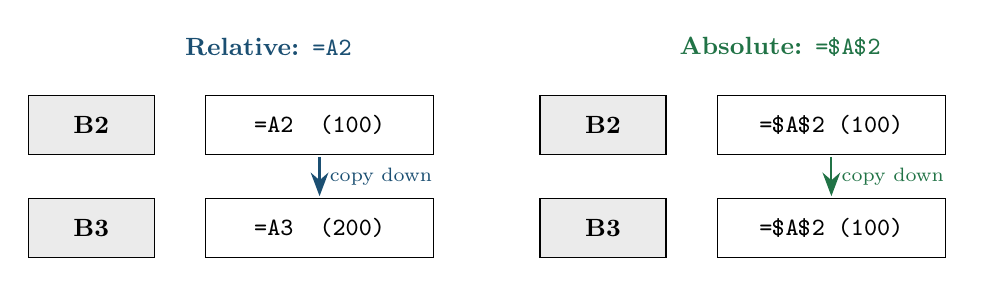
\begin{tikzpicture}[
  cell/.style={draw, minimum width=2.9cm, minimum height=0.75cm, font=\small\ttfamily, align=center},
  hdr/.style={draw, fill=black!8, minimum width=1.6cm, minimum height=0.75cm, font=\small\bfseries},
  lbl/.style={font=\small\bfseries}
]
\node[lbl, keyblue] at (2.25,3.0) {Relative: \texttt{=A2}};
\node[hdr] (rh1) at (0,2.0) {B2};
\node[cell] (rc1) at (2.9,2.0) {\texttt{=A2}\ \ (100)};
\node[hdr] (rh2) at (0,0.7) {B3};
\node[cell] (rc2) at (2.9,0.7) {\texttt{=A3}\ \ (200)};
\draw[-{Stealth[length=3mm]}, thick, keyblue] (2.9,1.6) to node[right, font=\scriptsize] {copy down} (2.9,1.1);

\node[lbl, excelgreen] at (8.75,3.0) {Absolute: \texttt{=\$A\$2}};
\node[hdr] (ah1) at (6.5,2.0) {B2};
\node[cell] (ac1) at (9.4,2.0) {\texttt{=\$A\$2}\ (100)};
\node[hdr] (ah2) at (6.5,0.7) {B3};
\node[cell] (ac2) at (9.4,0.7) {\texttt{=\$A\$2}\ (100)};
\draw[-{Stealth[length=3mm]}, thick, excelgreen] (9.4,1.6) to node[right, font=\scriptsize] {copy down} (9.4,1.1);
\end{tikzpicture}
\caption{Copying a formula one row down. The relative reference \texttt{A2} silently becomes \texttt{A3}, tracking the source data correctly in this case; the absolute reference \texttt{\$A\$2} deliberately refuses to move, always returning to the same fixed cell regardless of where the formula lives.}
\end{figure}

\subsection[The F4 Cycling Shortcut]{The \key{F4} Cycling Shortcut}

\begin{protip}[F4: Cycle Through Reference Types Without Retyping]
With the cursor positioned inside or immediately after a cell reference in the formula bar, pressing \key{F4} repeatedly cycles through all four states in a fixed order:
\begin{center}
\texttt{A1} $\rightarrow$ \texttt{\$A\$1} $\rightarrow$ \texttt{A\$1} $\rightarrow$ \texttt{\$A1} $\rightarrow$ \texttt{A1} $\rightarrow \cdots$
\end{center}
This is dramatically faster than manually typing \texttt{\$} symbols, especially inside a long formula with several references to lock, and is one of the highest-value habits to build early --- fluent Excel users use \key{F4} reflexively rather than typing dollar signs by hand.
\end{protip}

\subsection{Mixed References in Practice: A Two-Way Sensitivity Grid}

Mixed references exist for exactly one recurring scenario: a grid where \textbf{one axis should stay locked to a row, and the other axis should stay locked to a column} --- the classic use case being a sensitivity table with one assumption varying across the top and a second assumption varying down the side.

\begin{financeapp}[Revenue Sensitivity Grid]
Row 1 (\texttt{B1:E1}) holds four \textbf{base revenue} assumptions; column A (\texttt{A2:A5}) holds four \textbf{growth rate} assumptions. A single formula, typed once into \texttt{B2} and then copied across the \emph{entire} grid \texttt{B2:E5}, should correctly compute \emph{every} combination:
\end{financeapp}

\begin{formulasyntax}[The Grid Formula --- Typed Once Into B2]
\texttt{=B\$1*(1+\$A2)}
\begin{itemize}
  \item \texttt{B\$1} --- column \textbf{unlocked} (so it tracks whichever revenue column the formula currently sits under), row \textbf{locked} at \texttt{1} (so it always reads the header row, never a row of results).
  \item \texttt{\$A2} --- column \textbf{locked} at \texttt{A} (so it always reads the growth-rate column, never drifts right into the results), row \textbf{unlocked} (so it tracks whichever growth-rate row the formula currently sits in).
\end{itemize}
\end{formulasyntax}

\begin{center}
\begin{tabular}{@{}lcccc@{}}
\toprule
 & \textbf{B: 100} & \textbf{C: 150} & \textbf{D: 200} & \textbf{E: 250} \\
\midrule
\textbf{Row 2: 5\%}  & 105.0 & 157.5 & 210.0 & 262.5 \\
\textbf{Row 3: 10\%} & 110.0 & 165.0 & 220.0 & 275.0 \\
\textbf{Row 4: 15\%} & 115.0 & 172.5 & 230.0 & 287.5 \\
\textbf{Row 5: 20\%} & 120.0 & 180.0 & 240.0 & 300.0 \\
\bottomrule
\end{tabular}
\end{center}

\begin{keyconcept}
Every one of these 16 cells is the \emph{identical} formula text \texttt{=B\$1*(1+\$A2)} typed exactly once, then filled right and down --- the mixed locks do all the work of making the column reference track across and the row reference track down independently. Getting even one lock wrong (e.g., typing \texttt{\$B\$1} fully absolute) would make every cell in the grid read the same single revenue figure instead of tracking its own column, producing a grid that looks plausible at a glance but is silently wrong everywhere except column B.
\end{keyconcept}

\begin{protip}[Excel's Native ``Data Table'' Feature]
\textbf{What-If Analysis $\rightarrow$ Data Table} (Data tab) builds exactly this kind of two-way grid natively, without you writing the mixed-reference formula by hand --- you provide one formula referencing your model's live inputs, plus a row of column-input values and a column of row-input values, and Excel fills the grid by silently re-running the whole calculation once per cell. This is convenient, but recall the performance pitfall from \S\ref{sec:calcmode}: Data Tables recalculate on \emph{every} recalculation event by default and can become the single most expensive object in a model, which is precisely why \textbf{Automatic Except for Data Tables} exists as a calculation-mode option.
\end{protip}

\subsection{References Across Sheets and Workbooks}

The same \texttt{\$} locking applies identically to references that cross a sheet or workbook boundary:

\begin{formulasyntax}[Cross-Sheet and Cross-Workbook References]
\begin{itemize}
  \item Same workbook, another sheet: \texttt{='Assumptions'!\$B\$4} --- the sheet name is followed by \texttt{!}, and is wrapped in single quotes only if it contains a space or starts with a number.
  \item Another, currently open workbook: \texttt{='[Model.xlsx]Assumptions'!\$B\$4}.
  \item Another, closed workbook: identical syntax, but Excel additionally embeds the full file path, and the formula returns a cached last-known value until that workbook is next opened and refreshed.
\end{itemize}
\end{formulasyntax}

\begin{pitfall}[Revisiting the Tax-Rate Scenario]
Module 1 previewed this exact scenario: a tax-rate assumption sits in one cell, referenced by a formula in every row of a P\&L. Written with a relative reference (\texttt{=B10*TaxCell}) and copied down 50 rows, the reference to \texttt{TaxCell} silently drifts down 50 rows too --- by row 30 it may be reading a blank cell (silently returning \texttt{0}, no error at all) or, worse, a completely unrelated number that happens to sit in that position. The fix is either an absolute reference (\texttt{=B10*\$B\$4}) or, cleaner still, a \textbf{Named Range} (\texttt{=B10*TaxRate}) --- the subject of the next section, which solves this problem even more robustly by removing the raw cell address from the formula altogether.
\end{pitfall}

\subsection{Cross-Tool Translation: Python and SQL}

\begin{keyconcept}[Why This Problem Is Almost Unique to Excel]
Python and SQL do not really have an equivalent bug class here, and it's worth understanding precisely why. The entire relative/absolute distinction exists because Excel's mental model is ``write one formula, then \emph{copy} it many times, and let each copy silently adjust.'' Python's mental model is the opposite: you write \emph{one} operation and apply it to an entire column or table at once (\textbf{vectorisation}), so there is no ``copy'' step during which a reference could drift. A pandas operation like \texttt{df["Tax"] = df["Revenue"] * tax\_rate} runs once, references \texttt{tax\_rate} exactly once, and applies to every row simultaneously --- there is no analogue of accidentally letting \texttt{tax\_rate} drift to a different value on row 30, because there was never a per-row copy of the formula in the first place.
\end{keyconcept}

\begin{lstlisting}[style=pythonstyle, caption={The "always reference one fixed value" pattern, done the Python way -- a scalar constant, referenced once, broadcast automatically}]
import pandas as pd

df = pd.DataFrame({"Revenue": [100_000, 150_000, 200_000]})

TAX_RATE = 0.21   # a single, unambiguous, named constant -- the Python
                  # equivalent of what a Named Range achieves in Excel

# No "copying a formula down 50 rows" step exists here, so there is no
# reference to accidentally let drift -- pandas broadcasts the scalar
# across every row of the column in one call.
df["Tax"] = df["Revenue"] * TAX_RATE
print(df)
#    Revenue      Tax
# 0   100000  21000.0
# 1   150000  31500.0
# 2   200000  42000.0
\end{lstlisting}

SQL's story is similar, but worth stating precisely: a SQL table also has no concept of a copied formula ``drifting'', because a column's computed value (whether stored or computed on the fly in a query) is defined once, by name, and applies uniformly to every row that query touches.

\begin{lstlisting}[style=sqlstyle, caption={The same fixed-rate calculation in SQL -- a literal constant applied uniformly, or joined from a single-row config table}]
-- Option A: literal constant in the query itself
SELECT
    revenue,
    revenue * 0.21 AS tax
FROM company_financials;

-- Option B: a single-row "assumptions" table, joined in --
-- the SQL analogue of referencing a Named Range instead of
-- hard-coding the number, so the rate lives in exactly one place
SELECT
    f.revenue,
    f.revenue * a.tax_rate AS tax
FROM company_financials AS f
CROSS JOIN assumptions AS a;   -- assumptions has exactly one row
\end{lstlisting}

\begin{keyconcept}
The \texttt{CROSS JOIN} against a deliberately single-row \texttt{assumptions} table is the closest SQL gets to the Excel pattern of ``one cell that every row's formula reaches back to'' --- every output row is paired with the same one assumptions row, the same way every cell in a column referencing \texttt{\$B\$4} reaches back to the same one input cell. Both approaches share the same benefit over hard-coding the number directly: change the rate in exactly one place (the config table, or the referenced cell), and every dependent row updates correctly and simultaneously.
\end{keyconcept}

% ==================================================================
\section{Named Ranges}
\label{sec:namedranges}
% ==================================================================

\subsection{Why Named Ranges Exist}

\begin{keyconcept}[From Module 1 --- Now Fully Resolved]
Module 1 identified the core weakness of Excel's addressing system: a cell address like \texttt{C18} is \textbf{positional} --- ``third column, eighteenth row'' --- not \textbf{semantic}. It says nothing about what the cell actually represents. A \textbf{Named Range} lets you attach a meaningful, stable name to a cell or range, so a formula can say \texttt{=Revenue - COGS} instead of \texttt{=B10-B11}. This is the single biggest step toward making a formula \emph{self-documenting}: a reader (including you, six months later) can understand what a formula computes without first clicking every cell it references to discover what each one holds.
\end{keyconcept}

\subsection{Creating a Named Range}

\begin{formulasyntax}[Three Ways to Create a Name]
\begin{enumerate}
  \item \textbf{Name Box} (the small box at the far left of the formula bar, normally showing the active cell's address): select the range first, then click into the Name Box, type the name, and press \key{Enter}. The fastest method for a single, quick name.
  \item \textbf{Formulas $\rightarrow$ Define Name}: opens a dialog with explicit fields for Name, Scope, Comment, and the range itself (\textbf{Refers to}) --- preferred when you want to set the scope deliberately (\S\ref{sec:namescope}) or add a comment.
  \item \textbf{Formulas $\rightarrow$ Create from Selection}: select a range \emph{together with} its adjacent header row/column, and Excel automatically creates one name per data column (or row), using the header text as the name --- by far the fastest way to name an entire table's columns in one action.
\end{enumerate}
\end{formulasyntax}

\subsection{Naming Rules}

\begin{center}
\begin{tabular}{@{}L{4.4cm}L{7.4cm}@{}}
\toprule
\textbf{Rule} & \textbf{Detail} \\
\midrule
Must start with a letter or underscore & Cannot start with a number or most symbols. \\
No spaces & Use an underscore or CamelCase instead: \texttt{Tax\_Rate} or \texttt{TaxRate}, never \texttt{Tax Rate}. \\
Cannot look like a cell address & \texttt{Q3} is rejected, since it is indistinguishable from the cell address \texttt{Q3}; \texttt{Q3\_Revenue} is fine. \\
Case-insensitive & \texttt{TaxRate} and \texttt{taxrate} refer to the \emph{same} name --- Excel does not allow both to exist as distinct names simultaneously. \\
Reasonable length limit & Up to 255 characters, though names are conventionally kept short and readable. \\
\bottomrule
\end{tabular}
\end{center}

\subsection{Using a Named Range in a Formula}

Once defined, a name can be typed directly into any formula exactly like a cell reference, and --- critically --- \textbf{behaves as an absolute reference by default}: typing \texttt{TaxRate} into a formula and copying that formula anywhere else always resolves back to the same named cell, with no \texttt{\$} signs required at all.

\begin{lstlisting}[style=excelstyle, caption={Before and after naming a tax-rate assumption cell}]
Before:  =B10*$B$4
After:   =B10*TaxRate
\end{lstlisting}

\begin{financeapp}
Named ranges are also usable across sheets without repeating the sheet-name prefix: if \texttt{TaxRate} is defined at workbook scope (\S\ref{sec:namescope}) on an ``Assumptions'' tab, a formula on a completely different ``Income Statement'' tab can simply write \texttt{=Revenue*TaxRate}, with no \texttt{'Assumptions'!} prefix needed anywhere --- the name itself already knows where it points.
\end{financeapp}

\subsection{Scope: Workbook vs. Worksheet}
\label{sec:namescope}

Every name has a \textbf{scope}, set at creation time in the Define Name dialog:

\begin{itemize}
  \item \textbf{Workbook scope} (the default): the name is valid and resolves to the same cell from \emph{any} sheet in the workbook. Almost always what you want for a global assumption like a tax rate or a reporting currency.
  \item \textbf{Worksheet scope}: the name is only valid \emph{on that one sheet} --- using it from another sheet either produces an error or, more dangerously, silently refers to a \emph{different} name with the same text if one happens to exist at workbook scope or on the current sheet.
\end{itemize}

\begin{pitfall}[Scope Collisions]
A worksheet-scoped name can legally share the same text as a different worksheet-scoped name on another sheet --- for example, both a ``Q1'' tab and a ``Q2'' tab defining their own local name \texttt{StartDate}, each pointing at a different cell. This is occasionally useful (a template pattern repeated identically per tab) but is also a common source of confusion: a formula copied from the Q1 tab to the Q2 tab that references \texttt{StartDate} will silently resolve to the \emph{Q2} tab's own \texttt{StartDate}, not the one it originally pointed to, with no warning. When in doubt, prefer workbook-scoped names and give them specific, unambiguous text (\texttt{Q1\_StartDate}, \texttt{Q2\_StartDate}) instead.
\end{pitfall}

\subsection{The Name Manager}

\begin{formulasyntax}[Formulas $\rightarrow$ Name Manager \textnormal{(or} \key{Ctrl+F3}\textnormal{)}]
Opens a single dialog listing every defined name in the workbook, its scope, its current \textbf{Refers to} range, and any comment --- with buttons to \textbf{Edit} (redefine what a name points to, without touching any formula that uses it), \textbf{Delete}, or \textbf{Filter} the list (e.g. to show only names with errors). This is the single place to audit every name in a large model at once, and the first place to check when a formula referencing a name returns an unexpected result.
\end{formulasyntax}

\subsection{Named Ranges as Data Validation List Sources}

One of the most common practical uses of a named range is supplying the source list for a Data Validation dropdown (\S\ref{sec:datavalidation}) --- rather than typing a literal comma-separated list into the Data Validation dialog itself, you point it at a named range, so updating the named range's contents automatically updates every dropdown built from it, everywhere in the workbook.

\subsection{Dynamic Named Ranges and the Modern Alternative: Excel Tables}

A named range created via the Name Box or Define Name points to a \emph{fixed} address, such as \texttt{Assumptions!\$A\$2:\$A\$10}. If new rows are added below row 10, the name does not automatically grow to include them.

\begin{protip}[The Classic Fix --- OFFSET/COUNTA --- and Why It's Rarely Used Today]
Older Excel guidance defines a name whose \textbf{Refers to} field uses \texttt{OFFSET} combined with \texttt{COUNTA} to calculate a range's size dynamically, e.g. \texttt{=OFFSET(Assumptions!\$A\$2,\allowbreak0,0,\allowbreak COUNTA(Assumptions!\$A:\$A)-1,\allowbreak1)}, which grows or shrinks automatically as data is added or removed. This works, but \texttt{OFFSET} is \textbf{volatile} (\S\ref{sec:calcmode}) --- it forces a recalculation on every change anywhere in the workbook --- so this classic pattern has a real, measurable performance cost in a large model.
\end{protip}

\begin{keyconcept}[The Modern Answer: Excel Tables]
Selecting a data range and pressing \key{Ctrl+T} (or \textbf{Insert $\rightarrow$ Table}) converts it into an \textbf{Excel Table} --- a structured object that automatically expands its range as new rows are typed directly below it, carries its own \textbf{structured references} (\texttt{Table1[Revenue]} instead of \texttt{\$B\$2:\$B\$47}), and is \emph{not} volatile. A structured reference to a Table column is, for almost every practical purpose, a self-expanding named range without the \texttt{OFFSET} performance penalty, and is the modern, recommended replacement for dynamic named ranges in current Excel. It is introduced here because it depends conceptually on named ranges to understand, but a full treatment of Tables, structured references, and their interaction with lookup functions belongs alongside Module 3's lookup-function coverage.
\end{keyconcept}

\subsection{Named Constants: a Name With No Cell At All}

A name does not have to refer to a range --- the \textbf{Refers to} field in Define Name can instead hold a literal value or formula directly, with no cell reference at all:

\begin{lstlisting}[style=excelstyle, caption={Define Name dialog: Name = TaxRate, Refers to = 0.21 (no cell involved)}]
Name:        TaxRate
Refers to:   =0.21
\end{lstlisting}

\begin{keyconcept}
This is the Excel equivalent of a named constant in code (\texttt{TAX\_RATE = 0.21} in Python) --- useful for a value that is genuinely fixed and unlikely to need its own dedicated input cell (a rounding tolerance, a fiscal year-end month number), though most finance teams still prefer a visible input \emph{cell} for any assumption a user might reasonably want to change or audit, reserving named constants for true structural constants.
\end{keyconcept}

\subsection{Common Pitfalls}

\begin{pitfall}[\texttt{\#REF!} From Deleting a Named Range's Source]
Deleting the row or column a named range points to does \textbf{not} delete the name itself --- the name survives in the Name Manager but its \textbf{Refers to} field becomes \texttt{\#REF!}, and every formula using that name breaks simultaneously across the entire workbook. Always check the Name Manager before deleting rows/columns in a model that uses named ranges, and be aware that a single deletion can silently break formulas on sheets you weren't even looking at.
\end{pitfall}

\begin{pitfall}[Names Don't Follow a Copied Sheet the Way You'd Expect]
Copying an entire worksheet (right-click the sheet tab $\rightarrow$ \textbf{Move or Copy} $\rightarrow$ check \textbf{Create a copy}) duplicates any worksheet-scoped names defined on it, but workbook-scoped names are \emph{not} duplicated --- formulas on the copied sheet that reference a workbook-scoped name continue pointing back at the \emph{original} sheet's cell, not a new copy on the duplicated sheet. This is a frequent, confusing surprise when duplicating a monthly-report template.
\end{pitfall}

\subsection{Cross-Tool Translation: Python and SQL}

\begin{lstlisting}[style=pythonstyle, caption={Named ranges, the openpyxl way -- defined names actually written into the .xlsx file}]
from openpyxl import Workbook
from openpyxl.workbook.defined_name import DefinedName

wb = Workbook()
ws = wb.active
ws["A1"] = "TaxRate"
ws["B1"] = 0.21

# Registers a workbook-scoped name, exactly like Formulas -> Define Name --
# Excel itself will show "TaxRate" as a usable name when this file is opened.
wb.defined_names["TaxRate"] = DefinedName("TaxRate", attr_text="Sheet!$B$1")

ws["B2"] = "=B1*100000*TaxRate"   # a live formula string using the named range
wb.save("model.xlsx")
\end{lstlisting}

\begin{keyconcept}
In plain Python (outside an actual \texttt{.xlsx} file), the equivalent of a named range is simply a well-named \textbf{variable} --- \texttt{tax\_rate = 0.21} instead of a magic, unexplained \texttt{0.21} scattered through the code. This is such a basic, automatic habit in programming that it is easy to forget it is exactly the same discipline Excel needs deliberate effort (defining a name, remembering to use it instead of the raw cell) to achieve --- code enforces readable references by convention; Excel requires you to opt in.
\end{keyconcept}

SQL's closest equivalents are a \textbf{view} (a saved, named, reusable query definition) and a \textbf{CTE} (Common Table Expression, a name scoped to one query):

\begin{lstlisting}[style=sqlstyle, caption={A view: a persistent, named definition usable in any future query, like a workbook-scoped named range}]
CREATE VIEW high_value_expenses AS
    SELECT * FROM monthly_expenses WHERE amount > 20000.00;

-- Used later, by name, exactly like referencing TaxRate in a formula:
SELECT * FROM high_value_expenses WHERE category = 'Rent';
\end{lstlisting}

\begin{lstlisting}[style=sqlstyle, caption={A CTE: a name scoped only to the one query it's defined in, like a worksheet-scoped named range}]
WITH recent_expenses AS (
    SELECT * FROM monthly_expenses WHERE expense_date >= '2026-07-01'
)
SELECT category, SUM(amount)
FROM recent_expenses
GROUP BY category;
-- "recent_expenses" does not exist outside this one query,
-- just as a worksheet-scoped name does not exist outside its own sheet.
\end{lstlisting}

% ==================================================================
\section{Data Validation and Custom Validation Formulas}
\label{sec:datavalidation}
% ==================================================================

\subsection{Why Data Validation Exists}

\begin{keyconcept}
A blank Excel cell will accept absolutely anything typed into it --- a number where a date was expected, a negative value for a quantity that can never be negative, a free-text category that should have come from a fixed list of ten approved values. \textbf{Data Validation} (\textbf{Data} tab $\rightarrow$ \textbf{Data Validation}) lets you constrain, in advance, what a user is allowed to enter into a specific cell or range --- Excel's closest equivalent to a database \texttt{CHECK} constraint, and the only real defense a worksheet has against bad input at the point of entry, rather than discovering the bad data later when a formula downstream produces a wrong or broken result.
\end{keyconcept}

\subsection{The Data Validation Dialog: Three Tabs}

\begin{formulasyntax}[Data $\rightarrow$ Data Validation]
The dialog has three tabs, and a complete, professional validation rule normally uses all three together:
\begin{itemize}
  \item \textbf{Settings} --- defines the actual rule (what is and isn't allowed).
  \item \textbf{Input Message} --- an optional tooltip shown \emph{before} the user types anything, while the cell is simply selected.
  \item \textbf{Error Alert} --- what happens \emph{after} an invalid entry is attempted.
\end{itemize}
\end{formulasyntax}

\subsection{The Settings Tab: Allow Types}

\begin{center}
\begin{tabular}{@{}L{2.6cm}L{4.0cm}L{5.2cm}@{}}
\toprule
\textbf{Allow} & \textbf{Extra options} & \textbf{Typical use} \\
\midrule
Any value & --- & The default (no restriction) --- effectively ``no validation''. \\
Whole number & between / not between / equal to / greater than / less than (\ldots) a value or cell reference & Headcount, number of units, a year entered as \texttt{2026} rather than a date. \\
Decimal & Same comparison operators & A growth rate, a margin, any bounded numeric assumption. \\
List & A literal comma-separated list, \emph{or} a cell range/named range & The single most common rule in finance models: forcing a category, scenario name, or account type to come from a fixed, approved set (\S\ref{sec:dvlist}). \\
Date & between / not between / \ldots, comparing to a fixed date or another cell & A transaction date that must fall within the current fiscal period. \\
Time & Same comparison operators, for time-of-day values & Less common in finance; more typical in operational/scheduling sheets. \\
Text length & between / not between / \ldots, comparing character counts & Enforcing a fixed-length code (e.g. exactly 10-digit account numbers). \\
Custom & Any formula that evaluates to \texttt{TRUE} or \texttt{FALSE} & Any rule the built-in types can't express directly (\S\ref{sec:dvcustom}) --- the most powerful and most under-used option. \\
\bottomrule
\end{tabular}
\end{center}

\subsection{List Validation: Building a Dropdown}
\label{sec:dvlist}

\begin{formulasyntax}[List Validation --- Two Sources]
\begin{enumerate}
  \item \textbf{Literal list}: \textbf{Allow: List} $\rightarrow$ \textbf{Source}: type values directly, separated by commas, e.g. \texttt{Best Case,Base Case,Worst Case}. Quick, but the list is buried inside the dialog and must be edited there directly if it ever changes.
  \item \textbf{Range or Named Range source}: \textbf{Source}: reference a range, e.g. \texttt{=\$H\$2:\$H\$4}, or better, a \textbf{Named Range} (\S\ref{sec:namedranges}), e.g. \texttt{=ScenarioList}. Editing the named range's contents automatically updates \emph{every} dropdown built from it, everywhere in the workbook --- the clear best practice for any list likely to change or reused in more than one place.
\end{enumerate}
Checking \textbf{In-cell dropdown} (on by default) adds the small dropdown arrow that appears when the cell is selected; unchecking it still enforces the rule but with no visible arrow, occasionally used when a dropdown arrow would clutter a dense input area.
\end{formulasyntax}

\begin{financeapp}[Scenario Switches]
A dropdown list of \texttt{Best Case / Base Case / Worst Case}, sourced from a named range, feeding into an \texttt{INDEX}/\texttt{MATCH} or \texttt{XLOOKUP} formula (both covered in Module 3) that pulls the corresponding set of assumptions, is the standard mechanism behind an interactive ``scenario switch'' in a financial model --- letting a user flip the entire model's output between cases with one dropdown selection instead of manually overtyping a dozen assumption cells.
\end{financeapp}

\begin{financeapp}[Preventing Typos That Silently Break Aggregation]
A free-text ``Category'' column where one row is typed \texttt{"Rent"} and another is typed \texttt{"rent "} (trailing space) or \texttt{"Rentals"} will cause a \texttt{COUNTIF}/\texttt{SUMIF} (Module 3) grouping by category to silently split what should be one category into two or three, understating totals with no error message. Constraining that column to a List validation sourced from an approved category list eliminates this entire class of bug at the point of entry, rather than requiring after-the-fact data cleaning.
\end{financeapp}

\subsection{Whole Number, Decimal, Date, and Text Length Validation}

Each of these follows the same pattern: choose a comparison operator, then supply either literal values or --- more powerfully --- \textbf{cell references}, so the bound itself can be a live assumption rather than a hard-coded number.

\begin{lstlisting}[style=excelstyle, caption={A Decimal validation rule referencing a live cell as its upper bound, instead of a hard-coded number}]
Allow:     Decimal
Data:      between
Minimum:   0
Maximum:   =MaxGrowthRate      <- a Named Range, not a typed literal
\end{lstlisting}

\begin{financeapp}
Bounding a growth-rate input cell to, say, \texttt{0} to \texttt{50\%} prevents an obvious fat-finger entry (typing \texttt{500} meaning \texttt{5\%}, forgetting the cell is already formatted as a percentage) from silently flowing through an entire model and producing a wildly implausible --- but not obviously broken --- output.
\end{financeapp}

\subsection{Custom Validation: Writing Your Own Rule}
\label{sec:dvcustom}

\textbf{Allow: Custom} accepts any formula that evaluates to \texttt{TRUE} (entry allowed) or \texttt{FALSE} (entry rejected), evaluated as if it were typed into the \emph{first} cell of the validated range --- this is the closest Data Validation gets to writing arbitrary logic, and is what makes it genuinely powerful rather than just a set of preset dropdowns.

\begin{center}
\begin{tabular}{@{}L{4.6cm}L{6.6cm}@{}}
\toprule
\textbf{Goal} & \textbf{Custom formula (typed for the top-left cell of the range)} \\
\midrule
Prevent duplicate entries in a column & \texttt{=COUNTIF(\$A\$2:\$A\$100,A2)=1} \\
Only allow entry if another cell isn't blank & \texttt{=NOT(ISBLANK(\$B2))} \\
Restrict text to uppercase letters only & \texttt{=EXACT(A2,UPPER(A2))} \\
Cap a total column at a budget ceiling & \texttt{=SUM(\$C\$2:\$C2)<=\$BudgetCap} \\
Require text starting with a fixed prefix & \texttt{=LEFT(A2,3)="INV"} \\
\bottomrule
\end{tabular}
\end{center}

\begin{keyconcept}[Why the Reference Style Matters Here]
Custom validation formulas rely on exactly the relative/absolute reference distinction from \S\ref{sec:absrel}: notice \texttt{A2} (relative, so it correctly re-checks \emph{each row's own value} as the rule is applied down a column) against \texttt{\$A\$2:\$A\$100} (absolute, so the comparison range itself never shifts). Getting this wrong --- for instance, accidentally making the whole range relative too --- silently produces a duplicate-check that compares each row only to itself, which always evaluates \texttt{TRUE} and enforces nothing at all.
\end{keyconcept}

\subsection{Input Message and Error Alert}

\begin{formulasyntax}[Input Message Tab]
\textbf{Title} and \textbf{Input message} fields define a small tooltip that appears automatically whenever the cell is selected, \emph{before} anything is typed --- used to guide the user (``Enter a value between 0\% and 50\%'') rather than to police the entry after the fact.
\end{formulasyntax}

\begin{formulasyntax}[Error Alert Tab]
\textbf{Style} determines what happens on an invalid entry:
\begin{itemize}
  \item \textbf{Stop} --- rejects the entry outright; the user cannot leave the cell with invalid data in it. The strictest and most common choice for hard constraints.
  \item \textbf{Warning} --- shows a warning but lets the user override it and keep the invalid entry anyway (``Yes'' / ``No'' / ``Cancel''). Useful when a rule is a strong suggestion rather than an absolute requirement.
  \item \textbf{Information} --- simply informs the user, with no blocking behaviour at all; the entry is always accepted regardless.
\end{itemize}
\textbf{Title} and \textbf{Error message} customise the dialog text shown --- always worth writing a specific, helpful message (``Growth rate must be between 0\% and 50\%'') rather than leaving Excel's generic default, which merely says the value violates the rule defined for the cell without explaining what that rule actually is.
\end{formulasyntax}

\subsection{Circling Invalid Data}

\begin{protip}[Auditing Data That Was Already There]
Data Validation rules only intercept \emph{new} typed or pasted entries by default --- they do \textbf{not} retroactively check data that was already sitting in the cells before the rule was applied (a very common situation when validation is added to a sheet \emph{after} data has been pasted in from an external source). \textbf{Data $\rightarrow$ Data Validation $\rightarrow$ dropdown arrow next to Data Validation $\rightarrow$ Circle Invalid Data} draws a red circle around every existing cell in the workbook that currently violates its own validation rule, making it possible to audit and clean up pre-existing bad data in one pass rather than hunting for it manually.
\end{protip}

\subsection{Copying, Extending, and Removing Validation}

\begin{itemize}
  \item Data Validation is a cell \emph{property}, so it copies along with \textbf{Copy}/\textbf{Paste} (and with \textbf{Paste Special $\rightarrow$ Validation}, which pastes \emph{only} the rule, leaving the destination cells' existing values and formatting untouched).
  \item Applying a rule to an entire column (e.g. \texttt{C:C}) rather than just the currently-populated rows future-proofs the sheet against new rows added later --- at the cost of a very slightly larger workbook file, a trade-off almost always worth making for an input column.
  \item \textbf{Data $\rightarrow$ Data Validation $\rightarrow$ Clear All} removes the rule (and, separately, Input Message/Error Alert text) from the selected cells entirely.
\end{itemize}

\subsection{Cross-Tool Translation: Python and SQL}

\begin{lstlisting}[style=pythonstyle, caption={Data Validation, the openpyxl way -- rules written directly into the .xlsx so Excel itself enforces them on open}]
from openpyxl import Workbook
from openpyxl.worksheet.datavalidation import DataValidation

wb = Workbook()
ws = wb.active

# List validation, equivalent to Allow: List, Source: a literal list
dv_list = DataValidation(
    type="list",
    formula1='"Best Case,Base Case,Worst Case"',
    allow_blank=False,
    showErrorMessage=True,
    errorTitle="Invalid Scenario",
    error="Choose Best Case, Base Case, or Worst Case.",
)
ws.add_data_validation(dv_list)
dv_list.add("B2")

# Decimal validation, equivalent to Allow: Decimal, between 0 and 0.5
dv_decimal = DataValidation(
    type="decimal", operator="between", formula1="0", formula2="0.5",
    showErrorMessage=True, errorTitle="Out of Range",
    error="Growth rate must be between 0% and 50%.",
)
ws.add_data_validation(dv_decimal)
dv_decimal.add("B3")

wb.save("validated_model.xlsx")
\end{lstlisting}

\begin{keyconcept}[A Genuinely Different Philosophy: Prevent vs. Detect]
This is worth pausing on, because it is a real design-philosophy difference, not just a syntax difference. Excel's Data Validation is \textbf{preventative} --- it stops bad data from ever being entered into the cell in the first place. The default pandas/Python approach is usually \textbf{detective} --- data is loaded first, and \emph{then} checked, typically with an \texttt{assert} statement or a dedicated validation library:
\end{keyconcept}

\begin{lstlisting}[style=pythonstyle, caption={The pandas-native approach: validate after loading, not while typing}]
import pandas as pd

df = pd.read_csv("scenario_inputs.csv")

# Detective, not preventative -- this runs AFTER the data already
# exists in memory, and simply flags/raises if something is wrong.
assert df["growth_rate"].between(0, 0.5).all(), "Growth rate out of bounds!"
assert df["scenario"].isin(["Best Case", "Base Case", "Worst Case"]).all(), \
    "Unrecognised scenario value found!"
\end{lstlisting}

\begin{lstlisting}[style=pythonstyle, caption={A schema-based library (pandera) makes the same detective checks more declarative and reusable}]
# pip install pandera
import pandera as pa
from pandera import Column, Check

schema = pa.DataFrameSchema({
    "growth_rate": Column(float, Check.in_range(0, 0.5)),
    "scenario": Column(str, Check.isin(["Best Case", "Base Case", "Worst Case"])),
})

schema.validate(df)   # raises a detailed SchemaError if any row violates a rule
\end{lstlisting}

\begin{protip}[Choosing Based on Who Is Typing]
Excel's preventative style is the right choice whenever a \emph{human} is typing data directly into cells --- catching a mistake at the moment of entry is far more useful to that person than discovering it downstream. Python's detective style is the right choice for data arriving in bulk from a file, an API, or a database query, where there is no single ``moment of typing'' to intercept, and checking the whole batch at once after loading is both simpler and more thorough.
\end{protip}

SQL enforces constraints preventatively too, much closer in spirit to Excel's approach than pandas' after-the-fact checks:

\begin{lstlisting}[style=sqlstyle, caption={SQL constraints -- the direct equivalents of each Data Validation type}]
CREATE TABLE scenario_inputs (
    scenario     VARCHAR(20) NOT NULL
                 CHECK (scenario IN ('Best Case','Base Case','Worst Case')),
                 -- equivalent of Allow: List

    growth_rate  DECIMAL(5,4) NOT NULL
                 CHECK (growth_rate BETWEEN 0 AND 0.5),
                 -- equivalent of Allow: Decimal, between 0 and 0.5

    account_code CHAR(10) NOT NULL,
                 -- fixed length, equivalent of Allow: Text length, = 10

    entry_date   DATE NOT NULL
                 CHECK (entry_date >= '2026-01-01')
                 -- equivalent of Allow: Date, greater than a fixed date
);

-- Attempting to INSERT a row violating any CHECK is REJECTED by the
-- database itself -- exactly Data Validation's Stop-style Error Alert,
-- except it is enforced centrally for every application that ever
-- writes to this table, not just for someone typing in one worksheet.
INSERT INTO scenario_inputs VALUES ('Optimistic Case', 0.30, 'ACC0001234', '2026-08-01');
-- ERROR: new row violates check constraint on "scenario"
\end{lstlisting}

\begin{keyconcept}
A SQL \texttt{CHECK} constraint and an Excel Custom Data Validation formula are doing precisely the same conceptual job: rejecting a write that violates a business rule, enforced as close to the point of entry as the tool allows. The meaningful difference is scope --- a database constraint is enforced centrally, for \emph{every} application and user that ever writes to that table, whereas an Excel validation rule only protects the specific cells it was applied to, and can be bypassed entirely by pasting data into a \emph{different}, unvalidated cell and later copying it over --- worth remembering before treating Data Validation as a full substitute for careful data governance in a widely shared workbook.
\end{keyconcept}

% ==================================================================
\section{Worked Example: A Professional Assumptions Sheet in Three Tools}
% ==================================================================

Everything in this module, combined into one small but genuinely professional artifact: a scenario-driven assumptions block that is optimised, named, validated, and correctly generalises --- built identically in Excel, Python, and SQL.

\subsection{The Brief}

An ``Assumptions'' tab with: (1) a \textbf{Base Revenue} input and a \textbf{Tax Rate} input, each a Named Range; (2) a \textbf{Scenario} dropdown constrained by Data Validation to exactly three approved values, sourced from a Named Range; (3) a small two-way sensitivity grid showing projected after-tax profit across a range of revenue and growth-rate assumptions, built with correctly mixed references so one formula fills the entire grid; and (4) clean, gridline-free presentation formatting.

\subsection{Excel Implementation}

\begin{enumerate}
  \item \texttt{B2} holds \texttt{100000}, named \texttt{BaseRevenue} (Name Box); \texttt{B3} holds \texttt{0.21}, named \texttt{TaxRate}.
  \item \texttt{H2:H4} holds the three approved scenario names, named \texttt{ScenarioList} (Name Box, after selecting \texttt{H2:H4}).
  \item \texttt{B4} gets Data Validation: \textbf{Allow: List}, \textbf{Source: \texttt{=ScenarioList}}, Error Alert style \textbf{Stop}, with a custom message naming the three valid options.
  \item Row 6 (\texttt{C6:F6}) holds four growth-rate assumptions (\texttt{0\%}, \texttt{5\%}, \texttt{10\%}, \texttt{15\%}); column B (\texttt{B7:B10}) holds four revenue-multiplier scenarios. \texttt{C7} contains \texttt{=(\$B7*BaseRevenue)*(1+C\$6)*(1-TaxRate)}, filled across \texttt{C7:F10} --- one formula, correctly generalising across the whole grid via the mixed references \texttt{\$B7} and \texttt{C\$6}, exactly as in \S\ref{sec:absrel}.
  \item \textbf{View $\rightarrow$ Gridlines} unchecked; column B widened to fit \texttt{BaseRevenue}'s label; header row bolded.
\end{enumerate}

\begin{financeapp}
Notice \texttt{TaxRate} is used with \emph{no} \texttt{\$} signs at all inside the grid formula, and still behaves as a fully absolute reference everywhere it's copied --- this is the concrete payoff of \S\ref{sec:namedranges}'s claim that named ranges default to absolute behaviour, removing the need to remember \texttt{\$} for assumption cells at all.
\end{financeapp}

\subsection{Python Implementation}

\begin{lstlisting}[style=pythonstyle, caption={The full assumptions sheet, built end-to-end with openpyxl}]
from openpyxl import Workbook
from openpyxl.workbook.defined_name import DefinedName
from openpyxl.worksheet.datavalidation import DataValidation
from openpyxl.styles import Font

wb = Workbook()
ws = wb.active
ws.title = "Assumptions"
ws.sheet_view.showGridLines = False          # optimisation: clean presentation

# --- Inputs and named ranges ---
ws["A2"], ws["B2"] = "Base Revenue", 100000
ws["A3"], ws["B3"] = "Tax Rate", 0.21
ws["A4"], ws["B4"] = "Scenario", "Base Case"
wb.defined_names["BaseRevenue"] = DefinedName("BaseRevenue", attr_text="Assumptions!$B$2")
wb.defined_names["TaxRate"]     = DefinedName("TaxRate", attr_text="Assumptions!$B$3")

ws["H2"], ws["H3"], ws["H4"] = "Best Case", "Base Case", "Worst Case"
wb.defined_names["ScenarioList"] = DefinedName("ScenarioList", attr_text="Assumptions!$H$2:$H$4")

# --- Data validation, sourced from the named range, exactly like the Excel version ---
dv = DataValidation(type="list", formula1="=ScenarioList", allow_blank=False,
                     showErrorMessage=True, errorTitle="Invalid Scenario",
                     error="Choose Best Case, Base Case, or Worst Case.")
ws.add_data_validation(dv)
dv.add("B4")

# --- Two-way sensitivity grid: growth rates across, revenue multipliers down ---
growth_rates = [0.00, 0.05, 0.10, 0.15]
multipliers  = [0.8, 1.0, 1.2, 1.4]
for j, g in enumerate(growth_rates):
    ws.cell(row=6, column=3 + j, value=g)          # C6:F6
for i, m in enumerate(multipliers):
    ws.cell(row=7 + i, column=2, value=m)           # B7:B10

for i in range(4):
    for j in range(4):
        col_letter = chr(ord("C") + j)
        row_num = 7 + i
        # Same mixed-reference pattern as the Excel formula, written as a live string
        formula = f"=($B{row_num}*BaseRevenue)*(1+{col_letter}$6)*(1-TaxRate)"
        ws.cell(row=row_num, column=3 + j, value=formula)

ws["A1"].font = Font(bold=True)
wb.save("assumptions_sheet.xlsx")
\end{lstlisting}

\subsection{SQL Implementation}

\begin{lstlisting}[style=sqlstyle, caption={The same assumptions, expressed as governed, constrained tables}]
CREATE TABLE assumptions (
    key   VARCHAR(20) PRIMARY KEY,
    value DECIMAL(12,4) NOT NULL
);
INSERT INTO assumptions VALUES ('BaseRevenue', 100000), ('TaxRate', 0.21);

CREATE TABLE scenario_selection (
    scenario VARCHAR(20) NOT NULL
             CHECK (scenario IN ('Best Case', 'Base Case', 'Worst Case'))
             -- equivalent of the List Data Validation sourced from ScenarioList
);
INSERT INTO scenario_selection VALUES ('Base Case');

CREATE TABLE sensitivity_inputs (
    growth_rate DECIMAL(5,4) NOT NULL,
    multiplier  DECIMAL(5,4) NOT NULL
);
INSERT INTO sensitivity_inputs VALUES
    (0.00, 0.8), (0.05, 0.8), (0.10, 0.8), (0.15, 0.8),
    (0.00, 1.0), (0.05, 1.0), (0.10, 1.0), (0.15, 1.0),
    (0.00, 1.2), (0.05, 1.2), (0.10, 1.2), (0.15, 1.2),
    (0.00, 1.4), (0.05, 1.4), (0.10, 1.4), (0.15, 1.4);

-- The grid itself: a CROSS JOIN against the single-row assumptions,
-- exactly the pattern introduced at the end of S4 for "one shared input
-- every row reaches back to" -- SQL's answer to a named, absolute reference.
SELECT
    si.multiplier,
    si.growth_rate,
    (si.multiplier * rev.value) * (1 + si.growth_rate) * (1 - tax.value) AS after_tax_profit
FROM sensitivity_inputs AS si
CROSS JOIN (SELECT value FROM assumptions WHERE key = 'BaseRevenue') AS rev
CROSS JOIN (SELECT value FROM assumptions WHERE key = 'TaxRate') AS tax;
\end{lstlisting}

% ==================================================================
\section{Common Pitfalls \& Debugging Checklist}
% ==================================================================

\begin{center}
\begin{tabular}{@{}L{3.8cm}L{8.2cm}@{}}
\toprule
\textbf{Symptom} & \textbf{Likely cause \& fix} \\
\midrule
Macro that worked yesterday now does nothing to new rows & Recorded against a fixed range (\S\ref{sec:macrofix}) --- edit the code to compute the last row dynamically with \texttt{Cells(Rows.Count,\allowbreak"X").\allowbreak End(xlUp).\allowbreak Row} instead of a hard-coded address. \\
Macro is greyed out / workbook opened with a warning bar & Saved as \texttt{.xlsx} instead of \texttt{.xlsm} (macros silently stripped), or Trust Center macro settings are blocking execution (\S\ref{sec:macrosecurity}) --- re-save as \texttt{.xlsm} and/or click Enable Content only if the source is trusted. \\
A formula gives a wildly different, but plausible-looking, result after being copied & A relative reference that should have been absolute or mixed drifted (\S\ref{sec:absrel}) --- press \key{F4} on the offending reference and re-check which of the four states is actually needed. \\
A sensitivity/lookup grid is correct in one row or column but wrong everywhere else & One of the two mixed-reference locks was set backwards or made fully absolute (\S\ref{sec:absrel}) --- re-derive which axis needs the row lock and which needs the column lock. \\
Every formula referencing a named assumption suddenly shows \texttt{\#REF!} & The named range's source cell/row/column was deleted (\S\ref{sec:namedranges}) --- open the Name Manager (\key{Ctrl+F3}) to find and fix or re-point the broken name. \\
A dropdown shows the right values on one sheet but a stale or wrong list on a copied sheet & A workbook-scoped name did not duplicate the way expected when the sheet was copied (\S\ref{sec:namedranges}) --- verify in the Name Manager which sheet the name's \textbf{Refers to} field actually points to. \\
Old, clearly invalid data isn't circled even though Data Validation is applied & Validation only checks \emph{new} entries by default (\S\ref{sec:datavalidation}) --- use \textbf{Circle Invalid Data} to retroactively flag pre-existing bad values. \\
A large workbook has become sluggish, freezing for seconds after every keystroke & Likely volatile functions (\texttt{OFFSET}, \texttt{INDIRECT}, whole-column references) or automatic recalculation of a large Data Table (\S\ref{sec:calcmode}) --- switch to manual/Automatic-Except-Data-Tables calculation and audit for volatile functions. \\
\bottomrule
\end{tabular}
\end{center}

% ==================================================================
\section{Chapter Summary \& Self-Check}
% ==================================================================

Before moving to Module 3 (Excel Like a Pro), you should be able to, without looking anything up:

\begin{itemize}
  \item[$\square$] Explain the difference between cosmetic and performance optimisation, and name at least three settings/techniques for each.
  \item[$\square$] Use Text to Columns to split delimited text and to fix numbers stored as text, and explain why a macro built on it can silently stop covering new rows.
  \item[$\square$] Record a macro with both relative and absolute reference recording, explain the difference, and know when each is the correct choice.
  \item[$\square$] Save a macro-enabled workbook correctly as \texttt{.xlsm} and explain why a plain \texttt{.xlsx} save silently discards macros.
  \item[$\square$] Read a recorded VBA macro line by line and identify exactly which hard-coded range would break it if the dataset grew, then fix it using \texttt{Cells(Rows.Count,\allowbreak"X").End(xlUp).Row}.
  \item[$\square$] Write all four reference types (\texttt{A1}, \texttt{\$A\$1}, \texttt{\$A1}, \texttt{A\$1}) from memory, and cycle through them with \key{F4} without thinking about it.
  \item[$\square$] Build a two-way sensitivity grid with a single formula using correctly mixed references, filled across the whole grid.
  \item[$\square$] Create a Named Range via all three methods, explain workbook vs. worksheet scope, and know what breaks (and what doesn't) when its source is deleted.
  \item[$\square$] Build a Data Validation List dropdown sourced from a Named Range, plus at least one Custom formula-based validation rule.
  \item[$\square$] Explain, for each of the five topics in this module, its closest Python and SQL equivalent, and articulate \emph{why} several of these problems (reference drift especially) are largely unique to Excel's copy-based formula model.
\end{itemize}

% ==================================================================
\section{What's Next: Module 3 Preview}
% ==================================================================

Module 3, \textit{Excel Like a Pro}, builds directly on the named ranges and validated inputs from this module and covers:

\begin{itemize}
  \item \textbf{Find and Replace, Conditional Formatting} --- locating and bulk-editing data, and visually flagging values automatically based on rules (a native alternative to the VBA highlighting macro built in \S\ref{sec:macros}, for cases simple enough not to need code at all).
  \item \textbf{IF / Nested IF / IFS} --- branching logic inside a formula.
  \item \textbf{COUNTIF, AVERAGEIF, MAXIFS/MINIFS, SUMIF/SUMIFS} --- conditional aggregation, directly building on this module's Data Validation-enforced clean categories (\S\ref{sec:dvlist}) to avoid the typo-driven under-counting pitfall flagged there.
  \item \textbf{Error Handling} --- \texttt{IFERROR}, \texttt{IFNA}, and reading Excel's error codes (\texttt{\#REF!}, \texttt{\#N/A}, \texttt{\#DIV/0!}, \ldots), including the \texttt{\#REF!} case this module introduced via deleted named ranges.
  \item \textbf{VLOOKUP, HLOOKUP, XLOOKUP, INDEX/MATCH} --- retrieving data by a lookup key rather than a hard-coded position, replacing the last major category of positional fragility not yet solved by named ranges or Tables.
  \item \textbf{String Functions} --- \texttt{LEFT}, \texttt{RIGHT}, \texttt{MID}, \texttt{FIND}, \texttt{CONCATENATE}/\texttt{TEXTJOIN}, and others, extending the manual, one-time Text to Columns split from \S\ref{sec:texttocolumns} into live, formula-driven text manipulation.
\end{itemize}

\end{document}